\documentclass[12pt]{report}

% Packages
\usepackage[utf8]{inputenc} % For input encoding
\usepackage{graphicx} % For including images
\usepackage{setspace} % For setting line spacing
\usepackage{geometry} % For setting page margins
\usepackage{lipsum} % For generating placeholder text
\usepackage{natbib} % For bibliography
\usepackage{listings} % For code
\usepackage{xcolor}
\usepackage[ruled,vlined]{algorithm2e} % For pseudocode
\usepackage{amsmath} % For \text command
\usepackage{float} % For H option
\usepackage{amsthm}
\usepackage{tikz} % for trees

\theoremstyle{definition}
\newtheorem{definition}{Definition}[section]  % Define a new theorem environment called "definition"


% Page margins
\geometry{
    a4paper,
    left=1in,
    right=1in,
    top=1in,
    bottom=1in,
}

\lstset{
    language=Python,
    basicstyle=\ttfamily,
    keywordstyle=\color{blue},
    stringstyle=\color{orange},
    commentstyle=\color{green!70!black},
    showstringspaces=false,
    breaklines=true,
    breakatwhitespace=true,
    tabsize=4,
    numbers=left,
    numberstyle=\small\ttfamily\color{gray},
    frame=single,
}

\SetAlgoNlRelativeSize{-1}

\onehalfspacing

\title{\textbf{Dynamic Programming} \\
\Large{University College Cork}}
\author{Konrad Dagiel}
\date{April 2023}

\begin{document}

\maketitle

\chapter*{Abstract}
The outcome of this project is a self-contained, complete guide to dynamic programming which can 
be accessed by anyone online. The text serves to take a programmer with zero dynamic 
programming experience and give them a deep understanding of the topic, providing them with
enough comprehensive knowledge to solve dynamic programming problems on their own.
This project also proposes solutions to two new dynamic programming problems, The Interstellar Problem I and The Interstellar Problem II.

\chapter*{Declaration}
Declaration of Originality.\\
In signing this declaration, you are conforming, in writing, that the submitted work is entirely your own original work, except where clearly attributed otherwise, and that it has not been submitted partly or wholly for
any other educational award.\\
I hereby declare that:\\
• this is all my own work, unless clearly indicated otherwise, with full
and proper accreditation;\\
• with respect to my own work: none of it has been submitted at any educational institution contributing in any way to an educational award;\\
• with respect to another’s work: all text, diagrams, code, or ideas,\\
whether verbatim, paraphrased or otherwise modified or adapted, have\\
been duly attributed to the source in a scholarly manner, whether\\
from books, papers, lecture notes or any other student’s work, whether\\
published or unpublished, electronically or in print.\\
Signed: Konrad Dagiel\\
Date: 17/04/2024

\chapter*{Acknowledgements}
Dynamic Programming was originally proposed by Richard Bellman in the 1950s.
In Bellman's dynamic programming, problems are typically represented using states, actions, and transitions between states.
Each state represents a specific configuration or situation in the problem domain, and actions define the possible decisions or choices that can be made from each state.
This representation allows for a more structured approach to problem-solving and optimization.
Throughout this notebook when we refer to Dynamic Programming, we refer to a more general, modernized version of Dynamic Programming.

\tableofcontents

\chapter{Introduction}
\pagenumbering{arabic}
\setcounter{page}{1}
Dynamic programming is a powerful technique widely used in computer science for solving optimization and counting problems efficiently.
This project aims to address the challenge of creating an online course with the goal of teaching the dynamic programming technique in a way which can be easily digested by an average undergraduate computer science student.
The report contains detailed descriptions of eleven famous dynamic programming algorithms,
structured in a format which can be used as teaching material by a lecturer looking to give a class on dynamic programming to students with no prior knowledge of the technique.
Each of the problems include a Python implementation of the brute force, memoization and tabulation approach to the problem, a comprehensive and easily digestable complexity analysis of each of the approaches, as well as a rigorous comparative analysis of the runtimes of each of the approaches.
The code is accessible online for students looking to run it on their own inputs, and can be set to print the table it uses to arrive at the solution.
Finally, the project proposes a solution for two new dynamic programming problems, Python implementations of solutions to these problems, complexity analysis of these implementations, and a discussion of potential optimizations which could be made to make these solutions even more efficient.
 % intro to project

\chapter{Analysis} % what the project hopes to achieve

\chapter{Research on Dynamic Programming}

\section{Introduction to Dynamic Programming}
Dynamic Programming has many definitions, but can be summarized as a method of breaking down a larger problem into sub-problems, such that if you work through the sub-problems in the right order, building each answer on the previous one, you eventually arrive at a solution to the larger problem.
The two attributes a problem needs to have in order to be classified as a dynamic programming problem are as follows:

\begin{definition}[Optimal Substructure]
    A problem is said to have optimal substructure if an optimal solution to the problem can be deduced from optimal solutions of some or all of its subproblems.
\end{definition}

\begin{definition}[Overlapping Subproblems]
    A problem is said to have overlapping subproblems if the problem can be broken down into subproblems which can be reused several times, or a recursive algorithm would solve the same subproblem more than once resulting in repeated work. (If the subproblems do not overlap, the algorithm is categorized as a "divide and conquer" algorithm rather than a dynamic programming algorithm.)
\end{definition} 
Once we have deduced that a problem has both of these properties, we can use dynamic programming principles in order to solve the problem in an efficient manner.
When solving a dynamic programming problem, it is common to start by implementing a brute force solution which explores all subproblems and returns a solution.
We can then extend our solution to use a cache to store the results of any subproblems encountered, such that when the subproblem is encountered again we do not need to re-compute the result, instead we can simply look up the cache in constant time.
This is known as "memoization", or "top-down dynamic programming".
We can then look for any patterns in the cache table which, given an initialization (usually the base case of the recursive solution), would allow us to compute the values stored in the cache without ever traversing the decision tree of the problem itself.
This is known as "tabulation", or "bottom-up dynamic programming".
Finally, we can space optimize the cache to avoid storing information which is not needed to arrive at the solution.
This way, we arrive at the optimized dynamic programming solution to the problem.
In order to demonstrate this, we will use a simple problem called The Fibonacci Problem.

\section{The Fibonacci Problem}
\begin{description}
    \item[Problem Statement:]
        Compute $fib(n)$, the $n$'th number in the Fibonacci sequence. (Where $fib(1) = 1$, $fib(2) = 1$ and $fib(n) = fib(n-1) + fib(n-2)$.)
        
    \item[Input:] 
        A positive integer $n$.
        
    \item[Output:] 
        An positive integer $fib(n)$.
        
    \item[Example:]
        For: 

        $n = 7$
        
        $fib(n) = 13$

    \item[Explanation:]
        The Fibonacci sequence is as follows: 1,1,2,3,5,8,13,...\\
        We can see that the 7th number in the sequence is 13.

\end{description}


\subsection{Brute Force Approach to The Fibonacci Problem}

We will always start with a brute force approach, in which which will use recursion to explore all subproblems and arrive at the solution. 
We know that the base cases are $fib(1) = 1$ and $fib(2) = 1$.
By definition, we know that the recursive case is $fib(n) = fib(n-1) + fib(n-2)$.

A sample Python implementation is shown in Figure \ref{fig:fibonacci-bf}.

\begin{figure}[H]
    \centering
    \begin{lstlisting}
    def fib_bf(n):
        if n <=2: return 1
        return fib_bf(n-1) + fib_bf(n-2)
    \end{lstlisting}
    \caption{Fibonacci Brute Force Python Implementation}
    \label{fig:fibonacci-bf}
\end{figure}

In order to understand just how inefficent this approach is, consider the calculation of $fib(6)$.
Figure \ref{fig:fibonacci-bf-tree} shows the repeating subproblems, which share a color in the tree.
We can see that the amount of repeating subproblems would scale exponentially with $n$.

\begin{figure}[htbp]
    \centering
    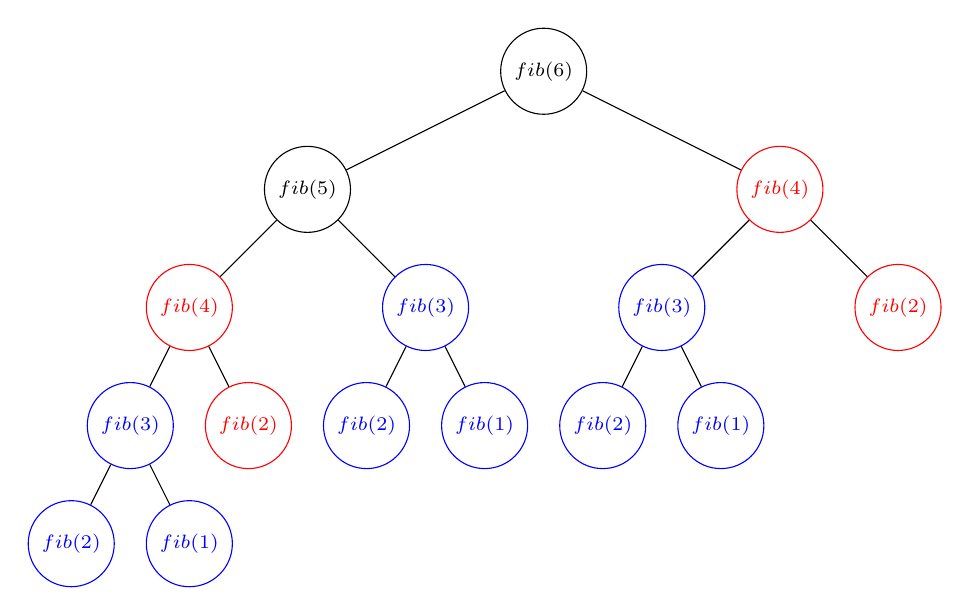
\begin{tikzpicture}[
        every node/.style={circle,draw,font=\scriptsize}, % Smaller font size
        level 1/.style={sibling distance=6cm},
        level 2/.style={sibling distance=3cm},
        level 3/.style={sibling distance=1.5cm}
    ]
        \node {$fib(6)$}
        child {node {$fib(5)$}
            child {node[red] {$fib(4)$}
                child {node[blue] {$fib(3)$}
                    child {node[blue] {$fib(2)$}}
                    child {node[blue] {$fib(1)$}}
                }
                child {node[red] {$fib(2)$}}
            }
            child {node[blue] {$fib(3)$}
                child {node[blue] {$fib(2)$}}
                child {node[blue] {$fib(1)$}}
            }
        }
        child {node[red] {$fib(4)$}
                child {node[blue] {$fib(3)$}
                    child {node[blue] {$fib(2)$}}
                    child {node[blue] {$fib(1)$}}
                }
                child {node[red] {$fib(2)$}}
            }
        ;
    \end{tikzpicture}
    
    \caption{Brute Force calculation of $fib(6) = 8$. Repeated subproblems share a color.}
    \label{fig:fibonacci-bf-tree}
\end{figure}

\subsection{Complexity Analysis of the Brute Force Approach to the Fibonacci Problem}

\begin{description}
    \item[Time Complexity:]
    At each step in the calculation of $fib(n)$, we make two 'branches', where one calculates $fib(n-1)$ and the other calculates $fib(n-2)$.
    This branching factor leads to an exponential growth in the number of function calls.
    The number of function calls grows exponentially with $n$, as each level of the tree doubles the number of function calls.
    Therefore the time complexity of this approach is $2 + 2^2 + 2^3 + ... + 2^n$ which is $O(2^n)$.
        
    \item[Space Complexity:] 
        In the brute force approach to The Fibonacci Problem, the space complexity is influenced by the recursive calls, each of which adds a frame to the call stack. However, as the recursion progresses, some of these frames can be discarded once their corresponding Fibonacci values have been computed.
        Specifically, at any point during the recursion, we only need to keep track of the previous two Fibonacci numbers. Therefore, the maximum depth of the call stack at any point is at most $n$ due to the recursion.
        This means that the space complexity of the brute force approach to compute Fibonacci numbers is $O(n)$.
        
        
    \item[Overall:] Total:\\
        Time Complexity: $O(2^n)$\\
        Space Complexity: $O(n)$
        
\end{description}
\newpage

\subsection{Memoization Approach to The Fibonacci Problem}
We can see that the optimal solution to $fib(n-1)$ + the optimal solution to $fib(n-2)$ will always be the optimal solution to $fib(n)$. This shows that the optimal substructure property holds.
We can also see that the calculation of $fib(n-1)$ contains the calculation of $fib(n-2)$, which is proof of overlapping subproblems.
This proves that The Fibonacci Problem fits the criteria for dynamic programming.
We can hence make this calculation more efficient through the use of memoization.
This simple adjustment involves storing a $(key, value)$ table called $memo$, where the key is an identifier for an intermediate subproblem and the value is the intermediate result of that subproblem.
Now, for any subproblem, we first check if the result is in $memo$ and if it is, we do not perform the calculation again, instead we return the result of that calculation from $memo$ in constant time.
If the subproblem is not in $memo$, we calculate the intermediate result and cache it in $memo$.

A sample Python implementation is shown in Figure \ref{fig:fibonacci-memo}.

\begin{figure}[H]
    \centering
    \begin{lstlisting}
    def fib_memo(n, memo={}):
        if n <= 2:
            return 1
        if n in memo:
            return memo[n]
        memo[n] = fib_memo(n-1, memo) + fib_memo(n-2, memo)
        return memo[n]
    \end{lstlisting}
    \caption{Fibonacci Memoization Python Implementation}
    \label{fig:fibonacci-memo}
\end{figure}

In the memoization solution, it is clear that we never repeat the calculation of a subproblem.
To visualize this, see Figure \ref{fig:fibonacci-memo-tree}, where repeated subproblems share a color.
We can see that we never repeat a calculation, as every time we visit a new node, we first check if it is present in $memo$, and if it is, we return the result immediately.
In this case, our $memo$ table key is $x$, and the value at $x$ returned is $fib(x)$.

\begin{figure}[H]
    \centering
    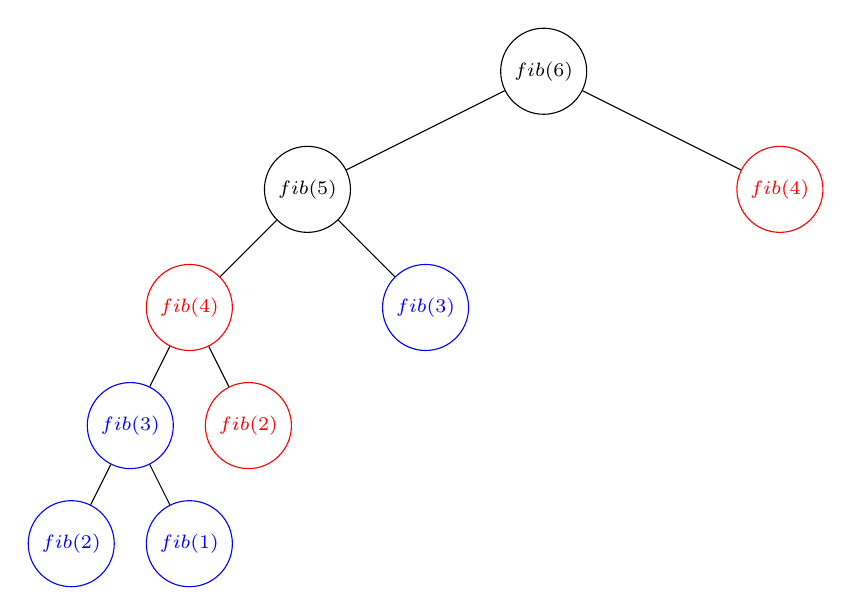
\begin{tikzpicture}[
        every node/.style={circle,draw,font=\scriptsize}, % Smaller font size
        level 1/.style={sibling distance=6cm},
        level 2/.style={sibling distance=3cm},
        level 3/.style={sibling distance=1.5cm}
    ]
        \node {$fib(6)$}
        child {node {$fib(5)$}
            child {node[red] {$fib(4)$}
                child {node[blue] {$fib(3)$}
                    child {node[blue] {$fib(2)$}}
                    child {node[blue] {$fib(1)$}}
                }
                child {node[red] {$fib(2)$}}
            }
            child {node[blue] {$fib(3)$}
            }
        }
        child {node[red] {$fib(4)$}
            }
        ;
    \end{tikzpicture}\\
    $memo$:
    \begin{table}[H]
        \centering
        \begin{tabular}{|c|c|c|c|c|c|c|}
            \hline
            \textbf{key:} & 1 & 2 & 3 & 4 & 5 & 6 \\
            \hline
            \textbf{value:} & 1 & 1 & 2 & 3 & 5 & 8 \\
            \hline
        \end{tabular}
    \end{table}
    \caption{Memoization calculation of $fib(6) = 8$. Repeated subproblems share a color.}
    \label{fig:fibonacci-memo-tree}
\end{figure}

\subsection{Complexity Analysis of the Memoization Approach to The Fibonacci Problem}

\begin{description}
    \item[Time Complexity:]
        Since each subproblem is only ever computed once, and any repeated subproblems are handled with a constant time table lookup,
        the time complexity depends only on the amount of subproblems.
        Since there are $n$ possible subproblems for any given input $n$,
        the time complexity is reduced to $O(n)$

    \item[Space Complexity:] 
        The space complexity remains determined by the recursion call stack, at $O(n)$.
        We also have to store the memo table, which contains an integer solution to each of the $n$ subproblems.
        This is also $O(n)$, giving us a total $O(2n)$ space complexity.
        This can be simplified to $O(n)$.

    \item[Overall:] Total:\\
        Time Complexity: $O(n)$\\
        Space Complexity: $O(n)$
        
\end{description}
\newpage

\subsection{Tabulation Approach to the Fibonacci Problem}
    
With the memoization approach, we saw how to compute the solution top-down, starting at $fib(n-1) + fib(n-2)$,
arriving at the base cases, and working up from there.
Notice that this step is unnecessary.
If we can deduce $fib(3)$ from $fib(2) + fib(1)$ (both of which are given in the base case),
and $fib(4)$ from $fib(3)$ and $fib(2)$,
we can work bottom-up until we arrive at $fib(n)$.
This is done by initializing an array of size $n$, placing 1 in the first and second cells as follows:
\begin{table}[H]
    \centering
    \begin{tabular}{|c|c|c|c|c|c|}
        \hline
        1 & 1 & \phantom{0} & \phantom{0} & \phantom{0} & \phantom{0} \\
        \hline
    \end{tabular}
\end{table}
And for each empty cell, filling it with the sum of the previous two cells.
This reduces the space complexity from $O(2n)$ to $O(n)$,
as all we need to do is store the table.
It is common practice to refer to the table as $dp$ in tabulation approaches.
Figure \ref{fig:fibonacci-dp-table} shows the complete $dp$ table.

\begin{figure}[H]
    \centering
    $dp$:
    \begin{table}[H]
        \centering
        \begin{tabular}{|c|c|c|c|c|c|}
            \hline
            1 & 1 & 2 & 3 & 5 & 8 \\
            \hline
        \end{tabular}
    \end{table}
    \caption{Tabulation Calculation of $fib(6)$.}
    \label{fig:fibonacci-dp-table}
\end{figure}

A sample Python implementation is shown in Figure \ref{fig:fibonacci-dp}.

\begin{figure}[H]
    \centering
    \begin{lstlisting}
    def fib_dp(n):
        if n <= 2:
            return 1

        dp = [1] * (n)

        for i in range(2, n):
            dp[i] = dp[i - 1] + dp[i - 2]

        return dp[n-1]
    \end{lstlisting}
    \caption{Fibonacci Tabulation Python Implementation}
    \label{fig:fibonacci-dp}
\end{figure}
\newpage

\subsection{Optimized Approach to the Fibonacci Problem}
We can often save space with the tabulation
approach by releasing parts of the $dp$ table which are not in use from memory.
In this case, notice that we only need $fib(n-1)$ and $fib(n-2)$ to deduce the result of $fib(n)$.
The rest of the table does not need to be stored. 
We can achieve this by storing just two variables, $prev$ and $curr$.
For an arbitrary value $x$, $curr$ represents the value of $fib(x)$, $prev$ represents the value of $fib(x-1)$.
We can calculate the result of $fib(x+1)$ from $prev$ and $curr$, then update $curr$ to the result, and $prev$ to what $curr$ was.
Starting at $curr=1$ and $prev=0$ and repeating this $n-1$ times will make $curr = fib(n)$.\\

A sample Python implementation is shown in Figure \ref{fig:fibonacci-optimized}.
\begin{figure}[H]
    \centering
    \begin{lstlisting}
    def fib_optimized(n):
        if n <= 1:
            return n
        
        prev, curr = 0, 1
        for _ in range(n-1):
            prev, curr = curr, prev + curr
            
        return curr
    \end{lstlisting}
    \caption{Fibonacci Optimized Python Implementation}
    \label{fig:fibonacci-optimized}
\end{figure}

\subsection{Complexity Analysis of the Tabulation Approach to the Fibonacci Problem}

\begin{description}
    \item[Time Complexity:]
        The time complexity remains unchanged at $O(n)$.

    \item[Space Complexity:] 
        Since we are only storing two variables of constant size at a time,
        and there is no recursion, the space complexity of this optimized version is $O(1)$.

    \item[Overall:] Total:\\
        Time Complexity: $O(n)$\\
        Space Complexity: $O(1)$
        
\end{description}
\newpage



\section{Dynamic Programming Summary}

In summary, the "dynamic programming way of thinking" involves:
\begin{enumerate}
    \item Creating a brute force solution.
    \item Figuring out if the optimal substructure property holds.
    \item Identifying the repeating and overlapping subproblems.
    \item Introducing memoization to the brute force solution to eliminate repeated work.
    \item Using tabulation to try to deduce the memoization table bottom-up rather than top-down.
    \item Looking for ways to optimize space in the tabulation approach by reducing the size of the table.
\end{enumerate}

Using the Fibonacci example, we have demonstrated the way of thinking about a problem which is dynamic programming.
We have went from an $O(2^n)$ time and $O(n)$ space complexity recursive solution to an $O(n)$ time and $O(1)$ space complexity solution using dynamic programming principles.
The Project Notebook contains an in depth analysis of 8 well known dynamic programming problems, followed by my own original dynamic programming problems and solutions.
Where applicable, the problems analyzed contain:

\begin{enumerate}
    \item The problem statement, and a deep explanation of the problem with examples. This may contain example greedy algorithms and proofs of why they do not actually work for the given problem.
    \item A comprehensive brute force algorithm, with an implementation and complexity analysis.
    \item A short informal proof of why the optimal substructure and overlapping subproblems attributes hold.
    \item An explanation of how memoization is used in the problem, with an implementation and complexity analysis.
    \item An explanation of how tabulation is used in the problem, with an implementation and complexity analysis.
    \item An explanation of how we can space optimize the tabulation solution, with an implementation and complexity analysis.

\end{enumerate}

In the Project Notebook, the tabulation approach of each of the problems comes with a $printTable$ flag which, when set to $True$, displays the table which has been calculated for the specific problem.

\section{The Coin Change Problem}
\begin{description}
    \item[Problem Statement:]
        Given a list of denominations of coins $D$ and an integer amount $a$, compute the minimum amount of coins (where each coin's denomination $\in D$) needed to sum exactly to the given amount $a$.
        
    \item[Input:] 
        An integer array $D$ of possible coin denominations, and an integer amount $a$.
        
    \item[Output:] 
        An integer $r$, which represents the minimum amount of coins with denominations $\in D$ needed in order to sum exactly to $a$. If this cannot be done, return $-1$.
        
    \item[Example:]
        For: 

        $D = [1, 5, 10, 20]$

        $a = 115$

        $r = 7$

    \item[Explanation:]
        The minimum amount of coins with denominations in $D$ needed to sum to $a$ is 7.

        These coins are: $[20,20,20,20,20,10,5]$


\end{description}

The problem appears trivial at first glance. One may be tempted to use a greedy method as follows:

\subsection{Greedy Approach to the Coin Change Problem}

Algorithm~\ref{algo:coin-change-greedy} shows a greedy approach to the coin change problem.

\begin{algorithm}[H]
    \caption{Greedy Approach to the Coin Change Problem}
    \label{algo:coin-change-greedy}
    \KwIn{List of denominations of coins $D$ and an amount $a$}
    \KwOut{$r$, The minimum number of coins required to make change for $a$}
    Sort $D$ in ascending order\;
    $r \leftarrow 0$\;
    $total \leftarrow 0$\;
    \While{$\text{total} < a$}{
        \If{$|D| = 0$}{
            \KwRet{-1}\;
        }
        \If{$\text{total} + D[-1] > a$}{
            $D.\text{pop()}$\;
        }
        \Else{
            $\text{total} \leftarrow \text{total} + D[-1]$\;
            $r \leftarrow r + 1$\;
        }
    }
    \KwRet{$r$}
\end{algorithm}

In Algorithm~\ref{algo:coin-change-greedy}, we always choose the coin with the largest value which will not make the total exceed a.

\subsection{Optimality of the Greedy Approach to the Coin Change Problem}

This algorithm is not optimal, and we can prove this by counter-example.\\
A counter example is $D = [5,4,3,2,1]$, $a = 7$.\\
Given these inputs, the greedy result is: $r1 = 3$  ([5,1,1]).\\
The optimal solution for these inputs is: $r2 = 2$ ([4,3]).\\
We see that $r1 > r2$, meaning the greedy approach does not find the miminized solution.\\

\subsection{Correctness of the Greedy Approach to the Coin Change Problem}

The greedy algorithm is also not correct, and we can prove this by another counter-example.\\
A counter example is $D = [4,3]$, $a = 6$.\\
Given these inputs, the greedy result is: $r1 = -1$  ([4]).\\
The optimal solution for these inputs is: $r2 = 2$ ([3,3]).\\
We see that the greedy approach fails when a solution is indeed possible, as shown by $r2$.\\
Since we have shown that the greedy approach is neither correct nor optimal, we move on to the brute force solution.\\


\subsection{Brute Force Approach to the Coin Change Problem}

The brute force approach to the coin change problem involves generating all possible coin combinations, and checking if any of them sum exactly to $a$.
Of the ones that do, we return the minimum length.\\
To try all possible coin combinations, we can subtract each coin denomination $c \in D$ from $a$, as long as $a - c >= 0$.\\
We can repeat this step for each result obtained from this calculation (replacing $a$ with the intermediate result), until all possible coin combinations are explored.\\
We can keep track of the shortest path through the resulting tree which has a leaf value of 0, to avoid storing the entire tree in memory.\\
We return the length of the shortest path as $r$.\\


% TODO NOTE: PLOT OF ALGORITHM HERE

A sample python implementation is shown in figure \ref{fig:coin-change-bf}.

\begin{figure}[h]
    \centering
    \begin{lstlisting}
    def coin_change_bf(D, a):
        def dfs(a):
            if a == 0:
                return 0
            if a<0:
                return float('inf')
            return min([1+dfs(a-c) for c in D])
        minimum = dfs(a)
        return minimum if minimum < float("inf") else -1
    \end{lstlisting}
    \caption{Coin Change Brute Force Python Implementation}
    \label{fig:coin-change-bf}
\end{figure}

\subsection{Complexity Analysis of the Brute Force Approach to the Coin Change Problem}

\begin{description}
    \item[Time Complexity:]
    For the worst case scenario, let's assume each coin denomination $c \in D < a$ such that each node which is not a leaf node has $|D|$ children. This means we have $|D|$ recursive calls at the first level, $|D|^{2}$ at the second level, $|D|^{n}$ at the $n$'th level.\\

    The total number of recursive calls in this scenario is $|D| + |D|^{2} + ... + |D|^{a}$ which is $O(|D|^a)$.
    
    Therefore the time complexity is $O(|D|^{a})$. This is because at each step, there are $|D|$ choices (coin denominations) to consider, and the recursion depth is at most $a$ (target amount).
    
        
    \item[Space Complexity:] 
        We do not store the entire tree in memory, only the current path.

        The space complexity is determined by the maximum depth of the recursion stack. In the worst case, the recursion depth is equal to the target amount $a$. Therefore, the space complexity is $O(a)$.
        
        
    \item[Overall:] total\\
        Time Complexity: $O(|D|^a)$

        Space Complexity: $O(a)$
        
\end{description}

\subsection{Memoization Approach to the Coin Change Problem}

In the brute force algorithm, we have a chance to arrive at a value multiple times. For every path in the search tree,
we can store intermediate results in a table which we will call $memo$ (for memoization) 
so that the next time we arrive at a value, eg. 3, we don't have to repeat the work in finding the minimum amount of extra coins needed to sum to $a$.
Instead we can simply look in the table with a constant time lookup.

This optimization reduces search time greatly, as seen in subsection \ref{subsec:ca-coin-change-memo}.

A sample python implementation is shown in figure \ref{fig:coin-change-memo}.

\begin{figure}[H]
    \centering
    \begin{lstlisting}
    def coin_change_memo(D, a):
    memo = {}
    def dfs(a):
        if a == 0:
            return 0
        if a < 0:
            return float('inf')
        if a in memo:
            return memo[a]
        
        memo[a] = min([1+dfs(a-c) for c in D])
        return memo[a]
            
    res = dfs(a)
    return res if res < float("inf") else -1
    \end{lstlisting}
    \caption{Coin Change Memoization Python Implementation}
    \label{fig:coin-change-memo}
\end{figure}

\subsection{Complexity Analysis of the Memoization Approach to the Coin Change Problem}\label{subsec:ca-coin-change-memo}

\begin{description}
    \item[Time Complexity:]
    %   CITATION HERE TO THE PYTHON MANUAL
        Each unique subproblem is evaluated once, and the next time it is encountered it is retrieved from the memoization table with a constant time lookup\footnote{Python dictionary lookups have an expected $O(1)*$ time complexity.}.
        As there are $|D| * a$ unique subproblems in the worst case\footnote{$|D|$ constant time subtractions from any intermediate value $v$ where $0 \leq v \leq a$.}, the time complexity to solve all of them is $O(|D| * a)$.
    
        
    \item[Space Complexity:] 
        We need to store the $memo$ table in memory.
        The memoization table is represented by a lookup data structure where the keys range from 0 to a,
        representing the solution to each unique subproblem.
        Hence, the memory required to store the table is of order $O(a)$.
        
    \item[Overall:] total\\
        Time Complexity: $O(|D| * a)$

        Space Complexity: $O(a)$
        
\end{description}

\subsection{Tabulation Approach to the Coin Change Problem}

Instead of doing a dfs to fill in the memo table, which requires a traversal of the exponential search tree, we can calculate the values in the memo table directly, and extract the answer from there.

We will call the $memo$ table $dp$, as we are no longer doing memoization, but tabulation.

$dp[i]$ represents the minimum amount of coins needed to get the amount $i$.

For the example $D = [5,4,3,1]$, $a = 7$

We initialize each $dp[i]$ to contain infinity.

We know that $dp[0] = 0$ as it takes $0$ coins to add up to an amount of $0$. We can initialize this in our table.

Now we can deduce $dp[1], dp[2], ... dp[a]$. $dp[a]$ will contain $r$.

To get $dp[i]$, we will look at each coin $c \in D$ in sequence.

For each $c \in D$, we take $i - c$ to get $t$, and look for $dp[t]$ if it exists.

Our intermediate result is $1 + dp[t]$

If this result is less than the current $dp[i]$ and is not negative, we update $dp[i] \leftarrow 1 + dp[t]$.

The logic of this is that the amount of coins it takes to make the amount $dp[i]$ is the amount of coins it takes to make the amount $dp[t]$ plus one.

The logic is demonstrated with the examples:

Example 1: Calculating $dp[1]$\\
$dp[0]=0$\\
$dp[1]=\infty$\\
$dp[2]=\infty$\\
$dp[3]=\infty$\\
$dp[4]=\infty$\\
$dp[5]=\infty$\\
$dp[6]=\infty$\\

To calculate $dp[1]$:

For $c \in D = [5,4,3,1]$

$t = i-c = 1-5 = -4$, ignore because negative

$t = i-c = 1-4 = -3$, ignore because negative

$t = i-c = 1-3 = -2$, ignore because negative

$t = i-c = 1-1 = 0$

Look up the value of $dp[t] = 0$.

Now we take $1 + dp[0] = 1$.

This means a possible solution to $dp[1]$ is 1.

Since $1 < \infty$, we update $dp[1] \rightarrow 1$

Example 2: Calculating $dp[7]$\\
$dp[0]=0$\\
$dp[1]=1$\\
$dp[2]=2$\\
$dp[3]=1$\\
$dp[4]=1$\\
$dp[5]=1$\\
$dp[6]=2$\\
$dp[7]=\infty$\\

To calculate $dp[7]$:

For each $c \in D = [5,4,3,1]$:

$t = i-c = 7-5 = 2$, $dp[2] = 2$, $1 + dp[2] = 3$, $3 < \infty$, update $dp[7] \rightarrow 3$

$t = i-c = 7-4 = 3$, $dp[3] = 1$, $1+dp[3] = 2$, $2 < 3$, update $dp[7] \rightarrow 2$

$t = i-c = 7-3 = 4$, $dp[4] = 1$, $1+dp[4] = 2$, $2 = 2$, ignore

$t = i-c = 7-1 = 6$, $dp[6] = 2$, $1+dp[6] = 3$, $3 > 2$, ignore

We conclude that the minimum solution to $dp[7] is 2$, achieved by adding a 4 coin to $dp[3]$, which is achieved by adding a 3 coin to $dp[0]$

A sample python implementation is shown in figure \ref{fig:coin-change-dp}.

\begin{figure}[H]
    \centering
    \begin{lstlisting}
    def coin_change_dp(D,a):
        dp=[float('inf')] * (a + 1)
        dp[0] = 0
    
        for i in range(1, a+1):
            for c in D:
                t = i - c
                if t >= 0:
                    dp[i] = min(dp[i], 1+dp[t])
    
        return dp[a] if dp[a] != float('inf') else -1
    \end{lstlisting}
    \caption{Coin Change Tabulation Python Implementation}
    \label{fig:coin-change-dp}
\end{figure}

\subsection{Complexity Analysis of the Tabulation Approach to the Coin Change Problem}

\begin{description}
    \item[Time Complexity:]
        % REFERENCE TO PYTHON MANUAL
        For the worst case scenario, we need to iterate for all $i = 0; i <= a; i++$.
        And for each $i$, we need to iterate over each coin $c \in D$.
        All other operations within the loops are constant time lookups and subtractions, so the time complexity is $O(|D| * a)$
            
    \item[Space Complexity:] 
        The space complexity is determined by the size of the $dp$ array. This array is always of size $a+1$.
        Therefore the space complexity is $O(a)$
        
    \item[Overall:] Total:\\
        Time Complexity: $O(|D| * a)$

        Space Complexity: $O(a)$
        
\end{description}

\section{Longest Increasing Subsequence}

\begin{description}
    \item[Problem Statement:]
        Given an array, return the length of the longest strictly increasing subsequence in the array.
        A sequence is said to be increasing if and only if \\$x1<x2<x3<...xn$.
        A subsequence does not have to be contiguous.

    \item[Input:]
        An integer array $nums$.
        
    \item[Output:]
        An integer $lis(nums)$, the length of the longest increasing subsequence of $nums$.
    \item[Example:] For:\\
        $nums = [2,5,3,7,101,18]$\\
        $lis(nums) = 4$

    \item[Explanation:]
    The subsequence $[2,5,7,101]$ is the longest increasing subsequence in $nums$, and has length $4$.

        
\end{description}

Much like coin change, this problem appears trivial at first glance. One may attempt to be greedy as follows:

\subsection{Greedy Approach to Longest Increasing Subsequence}

\begin{algorithm}
    \caption{Greedy Approach to Longest Increasing Subsequence}
    \label{algo:lis-greedy}
    \KwIn{An integer array $nums$.}
    \KwOut{An integer $lis$, the longest increasing subsequence in $nums$.}
    $lis \leftarrow 0$\;
    $index \leftarrow 0$\;
    $cur \leftarrow nums[0]$\;
    \While{$index \leq |nums|$}{
        \If{$nums[index] > cur$}{
            $lis += 1$\;
            $cur \leftarrow nums[index]$\;
        }
        $index +=1$\;
    }
    \KwRet{$lis$}
\end{algorithm}
In Algorithm \ref{algo:lis-greedy} we iterate through nums keeping track of the current max value enountered, incrementing our result each time a new larger value is encountered.

\subsection{Optimality of the Greedy Approach to Longest Increasing Subsequence}

This algorithm is not optimal however, and we can prove this by counter-example.
Take:$$nums = [10,9,2,5,3,7,101,18]$$
Given these inputs, the greedy result is: $r1 = 2  ([10,101])$.\\
An optimal solution for these inputs is: $r2 = 4 ([2,3,7,101])$.\\
We see that $r1 > r2$, meaning the greedy approach does not find the maximised solution.
We therefore need a more sophisticated approach.

\subsection{Brute Force Approach to Longest Increasing Subsequence}

We can try a brute force approach, where we start at $nums[0]$, and for each $i \in nums$ we generate two subsequences,
one where we  exclude $i$ from the subsequence and one where we include $i$ in the subsequence if
$nums[current\_index] > nums[prev\_index]$ (So that we ensure each subsequence generated is strictly increasing).
We keep track of the $prev\_index$, which represents the last index we included in the result,
and the $current\_index$, which is the index for which we are making the choice.
This will generate all possible increasing subsequenes.
We keep track of the length of the longest increasing subsequence, and return it once all increasing subsequences are explored.

A sample Python implementation is shown in Figure \ref{fig:lis-bf}.

\begin{figure}[H]
    \centering
    \begin{lstlisting}
    def lis_bf(nums):
        def dfs(prev_index, current_index):
            # Base case: reached the end of the sequence
            if current_index == len(nums):
                return 0
            # Case 1: Exclude the current element
            exclude_current = dfs(prev_index, current_index + 1)
            # Case 2: Include the current element if it is greater than the previous one
            include_current = 0
            if prev_index < 0 or nums[current_index] > nums[prev_index]:
                include_current = 1 + dfs(current_index, current_index + 1)
            # Return the maximum length of the two cases
            return max(exclude_current, include_current)
        # Start the recursion with initial indices (-1 represents no previous index)
        return dfs(-1, 0)
    \end{lstlisting}
    \caption{Longest Increasing Subsequence Brute Force Python Implementation}
    \label{fig:lis-bf}
\end{figure}

\subsection{Complexity Analysis of the Brute Force Approach to Longest Increasing Subsequence}
Let $n$ be the length of $nums$.
\begin{description}
    \item[Time Complexity:]
        For the worst case scenario, there are $n$ indices to consider.
        There are two subtrees at each decision, one where we include the current index, and one where we do not.
        This brings the time complexity to $O(2^n)$.
        
    \item[Space Complexity:] 
        The space complexity is determined by the recursion depth,
        as once we explore a path in the recursion tree, we can release it from memory when we go to the next path.
        Therefore the space complexity is $O(n)$.
        
        
    \item[Overall:] Total:\\
        Time Complexity: $O(2^n)$\\
        Space Complexity: $O(n)$
        

\end{description}


\subsection{Memoization Approach to Longest Increasing Subsequence}

Note that for an aribitrary longest increasing subsequence of length $k$ ending at index $i$,
if there exists exactly one number which can extend the sequence, the length of the total subsequence is guaranteed to be $k+1$.
This shows the optimal substructure property.
Also, when looking for subsequences at index $i$,
we must re-compute all of the subsequences at index $i-1$.
This shows the overlapping subproblems property.
We can use memoization to avoid repeating subproblems, such as when we are deciding wether the next element should be added or not for multiple subsequences ending in the same element.
The memoization approach goes as follows:
We initialize an empty dictionary called $memo$,
the keys of which are constructed by making a tuple of $(prev\_index, current\_index)$.
Before proceeding with the recursive calls, the function checks if the result for the current combination of $prev\_index$ and $current\_index$ is already computed and stored in the $memo$ dictionary.
If it is, the stored result is returned immediately.
This optimization allows the algorithm to avoid repeating work,
speeding up the runtime significantly.
Notice that memoization is not a space efficient approach to solving subsequence problems, as there is usually a lot of subproblems to store. In the case of longest increasing subsequence, memoization actually has a worse space complexity than the brute force approach.

A sample python implementation is shown in Figure \ref{fig:lis-memo}.

\begin{figure}[H]
    \centering
    \begin{lstlisting}
    def lis_memo(nums):
        if not nums:
            return 0
    
        memo = {}
    
        def dfs(prev_index, current_index):
            if current_index == len(nums):
                return 0
    
            if (prev_index, current_index) in memo:
                return memo[(prev_index, current_index)]
            
            exclude_current = dfs(prev_index, current_index + 1)
    
            include_current = 0
            if prev_index < 0 or nums[current_index] > nums[prev_index]:
                include_current = 1 + dfs(current_index, current_index + 1)
    
            memo[(prev_index, current_index)] = max(include_current, exclude_current)
    
            return memo[(prev_index, current_index)]
    
        return dfs(-1, 0)
    \end{lstlisting}
    \caption{Longest Increasing Subsequence Memoization Python Implementation}
    \label{fig:lis-memo}
\end{figure}

\subsection{Complexity Analysis of the Memoization Approach to Longest Increasing Subsequence}
Let n be the length of nums.
\begin{description}
    \item[Time Complexity:]
        For each unique combination of $(prev\_index, current\_index)$, the algorithm either calculates the result or looks it up in the $memo$ table.
        Each subproblem is calculated only once.
        The algorithm explores all combinations of $prev\_index$ and $current\_index$.
        There are at most $n$ choices for $current\_index$ and,
        in the worst case, $n$ choices for $prev\_index$ for each $current\_index$.
        Therefore, the total number of unique subproblems is $O(n^2)$.
        
    \item[Space Complexity:] 
        The space complexity is increased to $O(n^2)$,
        as the $memo$ table needs to store all $n^2$ combinations of $prev\_index$ and $current\_index$ in the worst case.
        
        
    \item[Overall:] Total:\\
        Time Complexity: $O(n^2)$\\
        Space Complexity: $O(n^2)$
    
\end{description}

\subsection{Tabulation Approach to Longest Increasing Subsequence}
We can use tabulation to build a table from which we can deduce the result, similar to the Coin Change Problem.
We know that a subsequence which consists of only the last index will result in an increasing subsequence of length 1.
We can work backwards, for the second last, third last ect.. deciding if including that element will result in a longer increasing subsequence or not,
and storing the longest possible increasing subsequence starting at each index until we reach index 0.
We create a table called $dp$ of size $|nums|$, where $dp[i]$ represents the longest increasing subsequence starting at index $i$ in nums.
Lets take the following example:$$nums = [1,2,4,3]$$
We initialize $dp[3] \leftarrow 1$, as the longest increasing subsequence starting at index 3 is 1.
\begin{table}[H]
    \centering
    $dp:$
    \begin{tabular}{|c|c|c|c|}
        \hline
        \phantom{0} & \phantom{0} & \phantom{0} & 1 \\
        \hline
    \end{tabular}
\end{table}
Now, consider $nums[2] = 4$
We can either take $nums[2]$ as a subsequence by itself, or include $nums[2]$ in any subsequence at any index that comes after it (as long as it maintains the property of an increasing subsequence).
Including it would make $dp[2] = 1+dp[3]$,
Excluding it would make $dp[2] = 1$.
Since including it would not result in an increasing subsequence, we must exclude it, so $dp[2] = 1$.
\begin{table}[H]
    \centering
    $dp:$
    \begin{tabular}{|c|c|c|c|}
        \hline
        \phantom{0} & \phantom{0} & 1 & 1 \\
        \hline
    \end{tabular}
\end{table}
Now Conisder $nums[1] = 2$.
We can either take it by itself or include it in any subsequence at any index that comes after it and maintains the increasing subsequence property.
Including it would make $dp[1] = max(1+dp[2], 1+dp[3])$, and taking it by itself would make $dp[1] = 1$.
We choose the option which maximizes the value of $dp[1]$, which is $1+dp[2]$ (or, equally, $1+dp[3]$) $= 2$.
\begin{table}[H]
    \centering
    $dp:$
    \begin{tabular}{|c|c|c|c|}
        \hline
        \phantom{0} & 2 & 1 & 1 \\
        \hline
    \end{tabular}
\end{table}
To generalize this, we set each $dp[i]$ to $max(1,1+dp[j1],1+dp[j2],1+dp[j3]...)$ where $jx$ is the index which comes $x$ places after $i$.
We only include $1+dp[jx]$ in the max function if $nums[i] < nums[jx]$, to maintain increasing subsequence property.
This will give us a table where $dp[i]$ contains the longest increasing subsequence of $nums$ where the first number is $nums[i]$.
We can then simply return $max(dp)$.\\

A sample python implementation is shown in Figure \ref{fig:lis-dp}.

\begin{figure}[H]
    \centering
    \begin{lstlisting}
    def lis_dp(nums):
        dp = [1] * len(nums)
    
        for i in range(len(nums)-1,-1,-1):
            for j in range(i+1,len(nums)):
                if nums[i] < nums[j]:
                    dp[i] = max(dp[i], 1+dp[j])
    
        return max(dp)
    \end{lstlisting}
    \caption{Longest Increasing Subsequence Tabulation Python Implementation}
    \label{fig:lis-dp}
\end{figure}

\subsection{Complexity Analysis of the Tabulation Approach to Longest Increasing Subsequence}
Let n be the length of nums.
\begin{description}
    \item[Time Complexity:]
        For the worst case scenario, we need to perform a double nested iteration over nums.
        All other operations within the loops are constant time, so the time complexity is of order $O(n^2)$.
        
    \item[Space Complexity:] 
        The space complexity is determined by the size of the $dp$ array. This array is always of size $n$.
        Therefore the space complexity is $O(n)$.
        
        
    \item[Overall:] Total:\\
        Time Complexity: $O(n^2)$\\
        Space Complexity: $O(n)$
    
\end{description}


\section{Max Subarray Sum}
\begin{description}
    \item[Problem Statement:]
        Given an integer array, return the largest value that a subarray\footnote{A subarray is a contiguous subsequence. This means all elements of the subsequence are strictly consecutive in the original sequence.} of the array sums to.

    \item[Input:]
        An integer array $nums$.
        
    \item[Output:]
        An integer $max\_sum$. 
        
    \item[Example:] For:\\
        $nums =  [-2,1,-3,4,-1,2,1,-5,4]$\\
        $max\_sum = 6$
        
    \item[Explanation:]
        $[4,-1,2,1]$ is the subarray of $nums$ that has the largest sum, 6.
        
\end{description}


\subsection{Brute Force Approach to Max Subarray Sum}
The naiive way to solve this problem is to generate every possible subarray of $nums$
starting with the subarray containing only $nums[0]$, and ending with the entirety of $nums$.
Then sum each subarray and get the maximum of these sums.
Instead of generating every subarray, we can iterate over each subarray in place by iterating over $nums$ with a $start$ pointer marking the start of the subarray,
and iterate over the rest of the array with an $end$ pointer marking the end of the subarray. This reduces the space complexity from O(n) to O(1) (see section \ref{subsec:ca-max-subarray-sum-bf}).
We can improve this further by keeping track of a $current\_sum$ and $max\_sum$ and updating them dynamically as we execute the $end$ loop rather than summing each subarray after it is generated,
reducing the time complexity from $O(n^3)$ to $O(n^2)$ (see section \ref{subsec:ca-max-subarray-sum-bf}).

A sample python implementation is shown in Figure \ref{fig:max-subarray-sum-bf}.

\begin{figure}[H]
    \centering
    \begin{lstlisting}
    def max_subarray_sum_bf(nums):
        if not nums:
            return 0
    
        n = len(nums)
        max_sum = float('-inf')
    
        for start in range(n):
            current_sum = 0
            for end in range(start, n):
                current_sum += nums[end]
                max_sum = max(max_sum, current_sum)
    
        return max_sum
    \end{lstlisting}
    \caption{Max Subarray Sum Brute Force Python Implementation.}
    \label{fig:max-subarray-sum-bf}
\end{figure}



\subsection{Complexity Analysis of the Brute Force Approach to Max Subarray Sum}\label{subsec:ca-max-subarray-sum-bf}
Let n be the length of nums.
\begin{description}
    \item[Time Complexity:]
        Due to the use of a double nested for loop,
        generating all subarrays of $nums$ has a time complexity of $O(n^2)$.
        All other operations such as adding to the $current\_sum$, resetting the $current\_sum$ and getting the max of $current\_sum$ and $max\_sum$ are constant time.
        If we were to sum each subarray individually rather than keeping a $current\_sum$, which would be an $O(n)$ operation, the total complexity would be increased to $O(n^3)$.

    \item[Space Complexity:] 
        All other variables stored such as $max\_sum$ and $current\_sum$ are constant space.
        The number of variables stored does not increase as $n$ increases, hence the space complexity is $O(1)$.
        If instead of iterating over each subarray in place, we stored the current subarray separately, the space complexity would be increased to $O(n)$.

    \item[Overall:] Total:\\
        Time Complexity: $O(n^2)$\\
        Space Complexity: $O(1)$
    
\end{description}

    
\subsection{Kadanes Algorithm for Max Subarray Sum}
    
There is a way to find the max subarray sum in a single iteration of $nums$.
This is done using the famous Kadane's algorithm.
Kadane's algorithm is shown in Algorithm \ref{algo:kadanes}: 

\begin{algorithm}[H]
    \caption{Kadane's Algorithm}
    \label{algo:kadanes}
    \KwIn{An integer array $nums$}
    \KwOut{An integer $max\_sum$, the max subarray sum of $nums$}
    $max\_sum = 0$\;
    $current\_sum = 0$\;
    \ForEach{$i \in nums$}{
        \If{$current\_sum < 0$}{
            $current\_sum := 0$\;
        }
        $current\_sum += i$\;
        \If{$current\_sum > max\_sum$}{
            $max\_sum := current\_sum$\;
        }
    }
    \KwRet{$max\_sum$}
\end{algorithm}
\subsection*{Explanation of Kadanes Algorithm}
In Kadane's algorithm, we iterate over $nums$, and at each step increment $current\_sum$ by the value of the current element. 
If $current\_sum$ becomes negative, $current\_sum$ is set to the value of current element. 
The $max\_sum$ is updated to $current\_sum$ whenever $current\_sum$ becomes greater than $max\_sum$.
If the array consists entirely of negative numbers, the algorithm will return 0 for the maximum subarray sum.
If you want to modify the algorithm such that empty subarrays are not allowed, you can initialize $max\_sum$ and $current\_sum$ to the first element of the array instead of 0.
This way, the algorithm will return the largest single negative element if the array consists entirely of negative numbers.
Kadane's algorithm is considered a dynamic programming algorithm even though it does not use a table, because it satisfies the necessary criteria:

Optimal Substructure: The problem of finding the maximum subarray can be divided into smaller subproblems, where the solution to the problem at each index depends on the solution to the problem at the previous index.

Overlapping Subproblems: The subproblems in Kadane's algorithm overlap, as the solution to the problem at each index relies on the solution to the problem at the previous index.

A sample python implementation is shown in Figure \ref{fig:kadanes}.

\begin{figure}[H]
    \centering
    \begin{lstlisting}
    def max_subarray_sum_kadanes(nums):
        if not nums:
            return 0
    
        max_sum = current_sum = nums[0]
    
        for num in nums[1:]:
            if current_sum < 0:
                current_sum = 0
            current_sum += num
            max_sum = max(max_sum, current_sum)
    
        return max_sum
    \end{lstlisting}
    \caption{Kadane's Algorithm Python Implementation}
    \label{fig:kadanes}
\end{figure}



\subsection{Complexity Analysis of Kadane's Algorithm}
Let n be the length of nums.
\begin{description}
    \item[Time Complexity:]
        This algorithm consists of a single iteration of nums, which is $O(n)$.
        All other operations such as updating the $current\_sum$, $max\_sum$ are constant time.
        
    \item[Space Complexity:] 
        All variables stored such as $max\_sum$ and $current\_sum$ are constant space,
        and we do not store more information as $n$ grows. Hence the space complexity is $O(1)$.

        
    \item[Overall:] Total:\\
        Time Complexity: $O(n)\\
        Space Complexity: $O(1)
    
\end{description}


\section{Longest Alternating Subsequence}
\begin{description}
    \item[Problem Statement:]
        Given an array, find the length of the longest alternating subsequence in the array.
        A sequence ${x1,x2,x3,x4...xn}$ is alternating if its elements satisfy one of the following:

        $x1>x2<x3>x4<...$
        
        $x1<x2>x3<x4>...$
        
    \item[Input:]
        An integer array $nums$.
        
    \item[Output:] 
        An integer $max\_length$.
        
    \item[Example:] For:\\
        $nums = [1,17,5,10,13,15,10,5,16,8]$\\
        $max\_length = 7$

    \item[Explanation:]
        The longest alternating subsequence in $nums$ is $[1,17,5,15,5,16,8]$ which has length $7$.

\end{description}

\subsection{Brute Force Approach to LAS}\label{subsec:las-bf}

The brute force way to approach this problem is to generate every possible subsequence of $nums$. 
For each subsequence, we can check if it is alternating iteratively, and if it is, calculate its length.
We keep track of the overall maximum length as we iterate through the subsequences. This way we are able to store just one subsequence at a time.

An implementation of the brute force algorithm is given in Figure \ref{fig:las-bf}.

\begin{figure}[H]
    \centering
    \begin{lstlisting}
    def is_alternating(sequence):
        if len(sequence) < 3:
            return True
    
        for i in range(1, len(sequence) - 1):
            if not ((sequence[i - 1] > sequence[i] < sequence[i + 1]) or
                    (sequence[i - 1] < sequence[i] > sequence[i + 1])):
                return False
        return True
    
    def las_bf(nums):
        if not nums:
            return 0
    
        n = len(nums)
        max_length = 1
    
        for i in range(1 << n):
            subsequence = [nums[j] for j in range(n) if (i & (1 << j)) > 0]
            if is_alternating(subsequence):
                max_length = max(max_length, len(subsequence))
    
        return max_length
    \end{lstlisting}
    \caption{Longest Alternating Subsequence Brute Force Python Implementation}
    \label{fig:las-bf}
\end{figure}


NOTE: In line 18 in Figure \ref{fig:las-bf}, The expression $1 << n$ represents a bitwise left shift operation.
In Python, $<<$ is the left shift operator, and it shifts the binary representation of the number to the left by $n$ positions.
In the context of generating all possible subsequences, $1 << n$ is used to create a bitmask with the rightmost $n$ bits set to $1$.
Each bit in the bitmask corresponds to whether the corresponding element in the array is included or excluded in the current subsequence.
The line "for $i$ in range$(1 << n)$" generates all possible subsequences by iterating through all bitmasks from 0 to $2^n-1$.

\subsection{Complexity Analysis of the Brute Force Approach to LAS}
Let n be the length of nums.
\begin{description}
    \item[Time Complexity:]
        The complexity of generating every possible subsequence is $O(2^n)$.
        Checking if a sequence is alternating is $O(|sequence|)$, which in the worst case is $n$,
        and getting the length of a subsequence, as well as comparing it to the $max\_length$ are $O(1)$.
        This is overall of order $O(2^n)$.
        
    \item[Space Complexity:] 
        The space complexity is $O(n)$, as we must store a single subsequence at a time,
        which in the worst case is of length $n$.
        
    \item[Overall:] Total:\\
        Time Complexity: $O(2^n)$\\
        Space Complexity: $O(n)$
    
\end{description}


\subsection{Auxiliary Arrays Solution for LAS}
Notice that for an aribitrary longest alternating subsequence of length $k$ ending at index $i$,
if there exists exactly one number which can extend the sequence,
the length of the total longest alternating subsequence is guaranteed to be $k+1$.
This shows the optimal substructure property.
Also, when looking for subsequences at index $i$,
we must re-compute all of the subsequences at index $i-1$.
This shows the overlapping subproblems property.

As using memoization on subsequence problems is not space efficient,
we can use tabulation and only store the necessary information rather than an intermediate result for every subsequence.
The following tabulation solution to Longest Alternating Subsequence is commonly referred to as the Auxiliary Arrays solution.

Two auxiliary arrays $inc$ and $dec$, of length $|nums|$ are initialized.
$inc[i]$ contains the length of the longest alternating subsequence of $nums[0:i]$,
where the last element of the subsequence is greater than the previous element.
$dec[i]$ contains the length of the longest alternating subarray of $nums[0:i]$,
where the last element of the subsequence is less than the previous element.\\

The algorithm iterates through $nums$, considering each element $nums[i]$ and updating the inc and dec arrays based on the following conditions:
\newpage

\begin{enumerate}
    \item If $nums[i]$ is greater than $nums[j]$ for some previous index $j$, it means the sequence can be extended in an increasing manner.
    In this case, $inc[i]$ is updated to be the maximum of its current value and the length of the longest decreasing subsequence ending at index $j+1$, found in $dec[j+1]$.

    \item If $nums[i]$ is smaller than $nums[j]$ for some previous index $j$, it means the sequence can be extended in a decreasing manner.
    In this case, $dec[i]$ is updated to be the maximum of its current value and the length of the longest increasing subsequence ending at index $j+1$, found in $inc[j+1]$.

    \item The length of the longest alternating subsequence is the maximum value in the $inc$ and $dec$ arrays.
\end{enumerate}


A sample Python implementation is shown in Figure \ref{fig:las-auxiliary}.

\begin{figure}[H]
    \centering
    \begin{lstlisting}
    def las_auxiliary(nums):
        n = len(nums)
        
        inc = [1] * n
        dec = [1] * n
    
        for i in range(1, n):
            for j in range(i):
                if nums[i] > nums[j]:
                    inc[i] = max(inc[i], dec[j] + 1)
                elif nums[i] < nums[j]:
                    dec[i] = max(dec[i], inc[j] + 1)

        return max(max(inc), max(dec))
    \end{lstlisting}
    \caption{Longest Alternating Subsequence Auxiliary Arrays Python Implementation}
    \label{fig:las-auxiliary}
\end{figure}
\newpage

\subsection{Complexity Analysis of the Auxiliary Arrays Approach to LAS}
Let n be the length of nums.
\begin{description}
    \item[Time Complexity:]
        We use a double nested for loop to iterate over $nums$.
        This gives a complexity of $O(n^2)$.
        All other operations are either constant time lookups, updates or $max(a,b)$,
        all of which are $O(1)$.
        
    \item[Space Complexity:] 
        The space complexity is $O(2n)$, which is of order $O(n)$.
        This is because we must store the $inc$ array and the $dec$ array,
        each of which have the same length as $nums$.
        All other variables are stored with constant space complexity.

        
    \item[Overall:] Total:\\
        Time Complexity: $O(n^2)$\\
        Space Complexity: $O(n)$
    
\end{description}


\subsection{Optimized Soluiton to LAS}
Observe that at each step, the max of $inc$ and $dec$ can be found at the current index of the arrays,
so we do not need to store the entire $inc$ and $dec$ arrays.
Instead, we can use an $inc$ and $dec$ variable which will hold the value stored at $inc[i]$ and $dec[i]$ respectively.
This is because a maximum alternating subsqeuence of $nums[0:a]$ will never be of lower length than a maximum alternating subsequence of $nums[0:b]$ if $a > b$.

We can do a single iteration over nums where:

\begin{enumerate}
    \item $inc$ should be set to $dec + 1$, if and only if the last element in the alternating sequence was less than its previous element.
    
    \item $dec$ should be set to $inc + 1$, if and only if the last element in the alternating sequence was greater than its previous element.

\end{enumerate}

A sample Python implementation is shown in Figure \ref{fig:las-optimized}.

\begin{figure}[H]
    \centering
    \begin{lstlisting}
    def las_optimized(nums):
        n = len(nums)
    
        inc = 1
        dec = 1
    
        for i in range(1, n):
            if nums[i] > nums[i - 1]:
                inc = dec + 1
            elif nums[i] < nums[i - 1]:
                dec = inc + 1
    
        result = max(inc, dec)
        return result
    \end{lstlisting}
    \caption{Longest Alternating Subsequence Optimzied Python Implementation}
    \label{fig:las-optimized}
\end{figure}

\subsection{Complexity Analysis of the Optimized Approach to LAS}
Let n be the length of nums.

\begin{description}
    \item[Time Complexity:]
        We use a single for loop to iterate over $nums$.
        This gives a complexity of $O(n)$.
        All other operations are either constant time lookups,
        updates or $max(a,b)$, all of which are $O(1)$.
        
    \item[Space Complexity:] 
        The space complexity is $O(1)$ as we only need to store a single value for $inc$ and $dec$.

    \item[Overall:] Total:\\
        Time Complexity: $O(n)$\\
        Space Complexity: $O(1)$
    
\end{description}

\newpage

\section{Binomial Coefficients}
\begin{description}
    \item[Problem Statement:]
        Given as input positive integers $n$ and $k$ where $n \geq k$, calculate how many different ways you can select $k$ unique examples from a set of size $n$.
        In other words, calculate $C(n,k)$ where: \[
            C(n,k) = \frac{n!}{k! \cdot (n-k)!}
            \]

    \item[Input:] 
        Two positive integers $n$ and $k$ where $n \geq k$.
        
    \item[Output:]
        A single positive integer $C(n,k)$.
        
    \item[Example:] For:\\
        $n = 4$\\
        $k = 2$\\
        $C(n,k) = 6$

    \item[Explanation:]
        There are 6 unique ways you can choose 2 different examples from a set of size 4.
        
\end{description}

We know that by definition:

$$C(n,k) = C(n-1,k-1) + C(n-1,k)$$

$$C(n,0) = 1$$

$$C(n,n) = 1$$

We can use this as a recursive case and base cases in a brute force solution.

\subsection{Brute Force Approach to Binomial Coefficients}
We can use recursion to arrive at our answer, using the definition as our recursive case and our base cases.

A sample Python implementation is shown in Figure \ref{fig:binomial-bf}.

\begin{figure}[H]
    \centering
    \begin{lstlisting}
    def C_bf(n,k):
        if k == 0 or k == n: return 1
        return C_bf(n-1,k-1) + C_bf(n-1,k)
    \end{lstlisting}
    \caption{Binomial Coefficients Brute Force Python Implementation}
    \label{fig:binomial-bf}
\end{figure}

\subsection{Complexity Analysis of the Brute Force Approach to Binomial Coefficients}
\begin{description}
    \item[Time Complexity:]
        For our analysis, in the worst case $k$ is equal to $n/2$.
        This means that at each recursion,
        we create two subproblems.
        We do this $n$ times, giving a total time complexity of $O(2^n)$.

    \item[Space Complexity:] 
        The space complexity is determined by the depth of recursion, which is $O(n)$.

    \item[Overall:] Total:\\
        Time Complexity: $O(2^n)$\\
        Space Complexity: $O(n)$
    
\end{description}

\subsection{Memoization Approach to Binomial Coefficients}
If we look at the trace of calculating $C(4,2)$ in our recursive algorithm, we can see that it is guaranteed to be the sum of $C(3,1)$ and $C(3,2)$, as by definition $C(n,k) = C(n-1,k-1) + C(n-1, k)$.
This shows the problem has the optimal substructure property.
To calculate $C(3,2)$ we must know $C(2,1)$.
This is also true when calculating $C(3,1)$.
This means there is repeated calculations of $C(2,1)$ when calculating $C(3,2)$,
showing the overlapping subproblems property.
In larger problems, the number of repeated calculations is vast.
We can use memoization to store each calculation we do in a table called $memo$ to avoid repeating subproblems.
At each step, before continuing with recursion, we check $memo$ to see if the calculation has been done already, and if so, we take the value from the $memo$ table instead of making a recursive call.\\

A sample Python implementation is shown in Figure \ref{fig:binomial-memo}.

\begin{figure}[H]
    \centering
    \begin{lstlisting}
    def C_memo(n,k,memo={}):
        if k == 0 or k == n: return 1
    
        if (n,k) in memo:
            return memo[(n,k)]
        
        result = C_memo(n-1,k-1,memo) + C_memo(n-1,k,memo)
        memo[(n,k)] = result
        return result
    \end{lstlisting}
    \caption{Binomial Coefficeints Memoization Python Implementation}
    \label{fig:binomial-memo}
\end{figure}

\subsection{Complexity Analysis of the Memoization Approach to Binomial Coefficients}
\begin{description}
    \item[Time Complexity:]
        The memoization table ensures that each unique subproblem is solved only once.
        In the case of $C(n,k)$ there are $O(n * k)$ unique subproblems because we must explore every combination of the parameters $n$ and $k$ in the worst case.
        The rest of the table lookups are expected constant time as we are using a dictionary for the $memo$ table.

    \item[Space Complexity:] 
        We must store the $memo$ table, which is a dictionary of size $O(n * k)$ as we must store every combination of $n$ and $k$.

    \item[Overall:] Total:\\
        Time Complexity: $O(n * k)$\\
        Space Complexity: $O(n * k)$
    
\end{description}

\subsection{Tabulation Approach to Binomial Coefficients}
Instead of recursively creating the table by searching the entire tree of possible $n$ and $k$ values, we can use tabulation to fill in a table from which we can extract our answer.
Consider a table $dp$ with dimensions ($n+1$) x ($k+1$), where $dp[i][j]$ in the table contains the result of $C(i,j)$
We could build this table up starting from our base cases:
$$C(n,0) = 1$$
$$C(n,n) = 1$$

until we have a solution to $C(n,k)$.

So for the calculation of $C(4,2)$ for example, we would initialize the following table:
(Note that the visualization of the table includes an additional row and column which contain labels in \textbf{bold} representing the possible values of $k$ and $n$ respectively. These are not part of the actual $dp$ table.)

\begin{table}[H]
    \centering
    \begin{tabular}{|c|c|c|c|}
        \hline
          & \textbf{0} & \textbf{1} & \textbf{2} \\
        \hline
        \textbf{0} & 1 & 0 & 0 \\
        \hline
        \textbf{1} & 1 & 1 & 0 \\
        \hline
        \textbf{2} & 1 &   & 1 \\
        \hline
        \textbf{3} & 1 &   &  \\
        \hline
        \textbf{4} & 1 &   &   \\
        \hline
    \end{tabular}
    \caption{Initialized $dp$ Table for $C(4,2)$}
\end{table}
Now, we can use $C(n,k) = C(n-1,k-1) + C(n-1,k)$ to fill the table.

For example, to get $dp[2][1]$ $(C(2,1))$, we take $dp[1][0] + dp[1][1] = 2$.

Do this for the entire table as follows:

\begin{table}[H]
    \centering
    \begin{tabular}{|c|c|c|c|}
        \hline
          & \textbf{0} & \textbf{1} & \textbf{2} \\
        \hline
        \textbf{0} & 1 & 0 & 0 \\
        \hline
        \textbf{1} & 1 & 1 & 0 \\
        \hline
        \textbf{2} & 1 & 2 & 1 \\
        \hline
        \textbf{3} & 1 & 3 & 3 \\
        \hline
        \textbf{4} & 1 & 4 & 6 \\
        \hline
    \end{tabular}
    \caption{Filled $dp$ Table for $C(4,2)$}
\end{table}

Until we arrive at $dp[n][k]$ which will give the answer of $C(n,k)$.\\

A sample Python implementation is shown in Figure \ref{fig:binomial-dp}.

\begin{figure}[H]
    \centering
    \begin{lstlisting}
    def C_dp(n,k):
        dp = [[0] * (k+1) for _ in range(n+1)]
    
        #Fill in the base cases
        for i in range(n+1):
            dp[i][0] = 1
            dp[i][min(i,k)]=1
    
        #Fill in the rest of the table using the definition of C(n,k)
        for i in range(1,n+1):
            for j in range(1,min(i,k)+1):
                dp[i][j] = dp[i-1][j-1] + dp[i-1][j]
                
        return dp[n][k]
    \end{lstlisting}
    \caption{Binomial Coefficients Tabulation Python Implementation}
    \label{fig:binomial-dp}
\end{figure}

NOTE: We do not fill the table where $k > n$.
This because it is impossible to choose $k$ unique examples from a set of size $n$.
This is done by only iterating to $min(i,k)$ in the inner loop, shown on line 11 of Figure \ref{fig:binomial-dp}.

\subsection{Complexity Analysis of the Tabulation Approach to Binomial Coefficients}

\begin{description}
    \item[Time Complexity:]
        We have to fill in a table of size $O(n * k)$ with values, and each value is obtained through a constant time lookup and addition.

    \item[Space Complexity:] 
        We must store the $dp$ table, which is a 2D array of size $O(n * k)$ as $n$ and $k$ can take values from $0$ to $n$.
        
    \item[Overall:] Total:\\
        Time Complexity: $O(n * k)$\\
        Space Complexity: $O(n * k)$
    
\end{description}

\subsection{Optimzied Tabulation Approach to Binomial Coefficeints}\label{subsec:binomial-coefficents-optimized}
Notice that we can calculate the values in any row $r$ using the values in row $r-1$.
Hence, we do not need to store the entire $dp$ table in memory, only two rows at a time.
The current row $r$, and the previous row $r-1$.
This reduces space complexity from $O(n * k)$ to $O(k)$.
Notice also that $C(n,k) = C(n,n-k)$.
We can therefore set $k = n-k$ if $k > n-k$ and $n-k$ is positive before we start our algorithm, and our result will be the same.
This reduces the time complexity from $O(n * k)$ to $O(n * min(k,n-k))$.\\

A sample Python implementation is shown in Figure \ref{fig:binomial-optimized}.

\begin{figure}[H]
    \centering
    \begin{lstlisting}
    def C_optimized(n,k):
        if k > n-k and n-k >= 0:
            k = n-k
        oldRow = [0] * (k+1)
        oldRow[0] = 1
    
        for i in range(1,n+1):
            newRow = [0] * (k+1)
            newRow[0] = 1
            for j in range(1,min(i,k)+1):
                newRow[j] = oldRow[j-1] + oldRow[j]
    
            oldRow = newRow
              
        return newRow[k]
    \end{lstlisting}
    \caption{Binomial Coefficients Optimized Python Implementation}
    \label{fig:binomial-optimized}
\end{figure}



\section{Longest Common Subsequence} \label{section:lcs}
\begin{description}
    \item[Problem Statement:]
        Given two strings, return the length of their longest common subsequence\footnote{Subsequences do not have to be contiguous.}.

    \item[Input:] 
        Two strings $text1$ and $text2$.
    \item[Output:] 
        An integer $lcs$, the longest common subsequence of $text1$ and $text2$.
        
    \item[Example:] For:\\
        $text1 = "abcde"$\\
        $text2 = "ace"$\\
        $lcs = 3$

    \item[Explanation:]
        The longest common subsequence of $"abcde"$ and $"ace"$ is $"ace"$, which is of length $3$.
   
\end{description}

\subsection{Longest Common Subsequence Brute Force}
The naiive way to find the longest common subsequence of two strings is to generate all possible subsequences of both strings.
We initialize a $lcs$ variable to store the length of the longest common subsequence.
We then iterate over each list of subsequences and report any common subsequences we find, updating $lcs$ accordingly.
Finally we return $lcs$.

\subsection{Complexity Analysis of the Brute Force Approach to Longest Common Subsequence}
For the calculation of worst case time and space complexity, we assume that both strings are equal in length, and that length is denoted by $n$.

\begin{description}
    \item[Time Complexity:]
        The time complexity of generating every subsequence of a string of length $n$ is $O(2^n)$,
        and doing this for both strings is $O(2 * (2^n))$ which is $O(2^n+1)$,
        as for each character we decide if we include it in or exclude it from the substring.
        The time complexity of iterating over two lists of substrings both of size $O(2^n)$ and looking for matches is $O((2^n)^2)$ which is equal to $O(2^{2n})$.
        This is still of order $O(2^n)$.

        
    \item[Space Complexity:]
        The space complexity of storing every subsequence of a string of length $n$ is $O(2^n)$.
        As we must do this for two strings, the total space complexity required is $O(2 * 2^n)$ which is of order $O(2^n)$.

    \item[Overall:] Total:\\
        Time Complexity: $O(2^n)$\\
        Space Complexity: $O(2^n)$
    
\end{description}

Notice that:

OBSERVATION 1: If we have a common character at the current position, such as position 1 in:

$$text1=abcde, text2=ace$$

The solution will be $1 + lcs(bcde,ce)$\footnote{Remove the common character from both texts, add 1 and recurse. The reason we add 1 is because each common character contributes 1 length to our final output.}.
This shows the problem has the optimal substructure property.

OBSERVATION 2: If there is no common character at the current position such as in:

$$text1=bcde, text2=ce$$

The solution will be $max(lcs(cde,ce), lcs(bcde,e))$\footnote{Remove the first character from either the first or second text, recurse on both cases.}.
As we have the chance to recurse on the same two substrings multiple times, the problem has the overlapping subproblems property.
\subsection{Tabulation Approach to Longest Common Subsequence}
We can use these two cases to solve this problem by tabulation.
We create a table called $dp$ with $i+1$ rows and $j+1$ columns, where $i$ and $j$ are the lengths of $text1$ and $text2$ respectively.
Each row and column of $dp$ represents a character in $text1$ and $text2$.

\begin{table}[htbp]
    \centering
    \begin{tabular}{|c|c|c|c|}
        \hline
          & \textbf{a} & \textbf{c} & \textbf{e} \\
        \hline
        \textbf{a} &   &   &   \\
        \hline
        \textbf{b} &   &   &    \\
        \hline
        \textbf{c} &   &   &    \\
        \hline
        \textbf{d} &   &   &   \\
        \hline
        \textbf{e} &   &   &    \\
        \hline
    \end{tabular}
\end{table}

In this table, for example,
$dp[0][0]$ will represent $lcs(abcde,ace) \rightarrow$  the solution.
$dp[3][1]$ will represent $lcs(de,ce)$ ect..
i.e. $dp[i][j]$ represents the longest common subseqence of $text1[i:]$ and $text2[j:]$.

We fill the table starting from the bottom right as follows:

\begin{enumerate}
    \item If the row and column have the same label, we have found a common character.

    As per OBSERVATION 1, we fill the space with $1 + dp[i+1][j+1]$.
    
    \item If the row and col do not have the same label, we must use OBSERVATION 2:

    Fill the space with $max(dp[i][j+1], dp[i+1][j])$.
    
    \item If we go out of bounds, we simply take zero\footnote{For ease of code, the grid is ($i+1$) x ($j+1$) and initialized to all zeros, so we don't have to check for going out of bounds.}.
\end{enumerate}

Our solution will be located at $dp[0][0]$, which represents $lcs(text1,text2)$.

\begin{table}[htbp]
    \centering
    \begin{tabular}{|c|c|c|c|}
        \hline
          & \textbf{a} & \textbf{c} & \textbf{e} \\
        \hline
        \textbf{a} & 3 & 2 & 1 \\
        \hline
        \textbf{b} & 2 & 2 & 1  \\
        \hline
        \textbf{c} & 2 & 2 & 1  \\
        \hline
        \textbf{d} & 1 & 1 & 1 \\
        \hline
        \textbf{e} & 1 & 1 & 1  \\
        \hline
    \end{tabular}
\end{table}



A sample python implementation is shown in Figure \ref{fig:lcs-dp}.

\begin{figure}[H]
    \centering
    \begin{lstlisting}
    def lcs(text1, text2):
        dp=[[0 for j in range(len(text2)+1)] for i in range(len(text1)+1)]
    
        for i in range(len(text1)-1,-1,-1):
            for j in range(len(text2)-1,-1,-1):
                if text1[i] == text2[j]:
                    dp[i][j] = 1 + dp[i+1][j+1]
                else:
                    dp[i][j] = max(dp[i][j+1], dp[i+1][j])
    
        return dp[0][0]
    \end{lstlisting}
    \caption{Longest Common Subsequence Tabulation Python Implementation}
    \label{fig:lcs-dp}
\end{figure}

\subsection{Complexity Analysis of the Tabulation Approach to Longest Common Subsequence}

Let $i$ be the length of $text1$, and $j$ be the length of $text2$.

\begin{description}
    \item[Time Complexity:]
        The time complexity of filling an $i * j$ table with values, where each value is derived from a constant time lookup and a constant time addition or max function is $O(i * j)$.

    \item[Space Complexity:] 
        The space complexity of storing an $i * j$ table is $O(i * j)$.

        
    \item[Overall:] Total:\\
        Time Complexity: $O(i * j)$\\
        Space Complexity: $O(i * j)$
    
\end{description}

NOTE THAT SINCE EACH ROW OF THIS TABLE CAN BE COMPUTED USING THE PREVIOUS ROW ONLY, THE SAME TWO-ROW METHOD CAN BE USED AS IN BINOMIAL COEFFICIENTS

\section{Longest Palindromic Subsequence}
\begin{description}
    \item[Problem Statement:]
        Given a string, return the length of the longest subsequence\footnote{Subsequences do not have to be continuous.} of the string which is a palindrome\footnote{A palindrome is a string which is identical to itself when reversed (Example: "racecar").}.
    
    \item[Input:]
        A string $s$.
        
    \item[Output:]
        An integer $lps$ which represents the longest palondromic subsequence of $s$.
        
    \item[Example:] For:\\
        $s = "babbb"$\\
        $lps = 4$
        
    \item[Explanation:]
        $"bbbb"$ is the longest palindromic subsequence of $s$. It has length $4$.
\end{description}

\subsection{Tabulation Approach to Longest Palindromic Subsequence}
This problem is simply a special case of Longest Common Subsequence.
The longest palindromic subsequence of $s$ is simply the longest common subsequence of $s$ and $reverse(s)$.
Therefore the same logic applies. See Section \ref{section:lcs}.

A sample python implementation is shown in Figure \ref{fig:lps-dp}.
For the implementation of the lcs subroutine, see Figure \ref{fig:lcs-dp}.

\begin{figure}[H]
    \centering
    \begin{lstlisting}
    def lps(s):
        return lcs(s,s[::-1])
    \end{lstlisting}
    \caption{Longest Palindromic Subsequence Python Implementation}
    \label{fig:lps-dp}
\end{figure}

\section{Longest Contiguous Palindromic Substring}
\begin{description}
    \item[Problem Statement:]
        Given a string, return the longest contiguous palindromic substring of the string.

    \item[Input:] 
        A string $s$.
        
    \item[Output:] 
        A string $lpcs(s)$, which is the longest contiguous palindromic substring of $s$.
        
    \item[Example:] For:\\
        $s = "aaaabbaa"$\\
        $lpcs(s) = "aabbaa"$

    \item[Explanation:]
        The longest palindromic substring of $"aaaabbaa"$ is $"aabbaa"$.
        Note that here we are asked for the substring itself, rather than the length of the substring.
   
\end{description}

\subsection{Brute Force Approach to Longest Contiguous Palindromic Substring}
If we were to tackle this problem the brute force way, we would have to iterate over all substrings of s, filtering out non palindromes along the way,
and keeping track of the longest palindromic substring found so far. 
We would then return the longest palindromic substring of s.

\subsection{Complexity Analysis of the Brute Force Approach to Longest Contiguous Palindromic Substring}
Let n be the length of s.

\begin{description}
    \item[Time Complexity:]
        Iterating over all substrings of a string of length $n$ has a time complexity of $O(n^2)$.
        Checking if a substring is a palindrome has a time complexity of $O(n)$.
        This gives the brute force approach an overall time complexity of $O(n^3)$.
        
    \item[Space Complexity:] 
        The space complexity of generating all substrings and storing them in a list is also $O(n^3)$
        because we have $O(n^2)$ substrings, each of which has a maximum length of $O(n)$.
        However, in our algorithm it is possible to iterate over the subsrtings of $s$ in place using a double for loop
        like in Figure \ref{fig:max-subarray-sum-bf}. This brings the space complexity down to $O(n)$.
        
    \item[Overall:] Total:\\
        Time Complexity: $O(n^3)$\\
        Space Complexity: $O(n)$
    
\end{description}
Notice that if a string $p$ is a palindrome, and $x$ is a character, the string $xpx$ is guaranteed to be a palindrome.
This is proof of optimal substructure.
The problem of determining whether a substring is a palindrome or not can be reduced to smaller subproblems.
For example, when checking if $s[i:j]$ is a palindrome, we often need to check if $s[i+1:j-1]$ is a palindrome,
which overlaps with other similar subproblems.
Therefore, we can use dynamic programming principles to optimize the solution to this problem.
\subsection{Tabulation Approach to Longest Contiguous Palindromic Substring.}
We can create a table $dp$ where $dp[i][j] = 1$ if $s[i:j+1]$ is a palindrome, else 0. (eg: if $dp[1][3] = 1$, $s[1:4] (\text{"aaa" in our example string})$ is a palindrome.)
We start with a table $dp$ which is a 2D matrix of size $|s| * |s|$.
We can initialize all fields where $i == j$ to 1, as all single letter substrings are palindromes by definition. (Note that the below table has an extra row and column containing labels for each of the other rows and columns in the table. These are not part of the $dp$ table and are included in the figure for clarity.)

\begin{table}[htbp]
    \centering
    \begin{tabular}{|c|c|c|c|c|c|c|c|c|}
        \hline
          & \textbf{a} & \textbf{a} & \textbf{a} & \textbf{a} & \textbf{b} & \textbf{b} & \textbf{a} & \textbf{a} \\
        \hline
        \textbf{a} & 1 &  &  &  &  &  &  &  \\
        \hline
        \textbf{a} &  & 1 &  &  &  &  &  &  \\
        \hline
        \textbf{a} &  &  & 1 &  &  &  &  &  \\
        \hline
        \textbf{a} &  &  &  & 1 &  &  &  &  \\
        \hline
        \textbf{b} &  &  &  &  & 1 &  &  &  \\
        \hline
        \textbf{b} &  &  &  &  &  & 1 &  &  \\
        \hline
        \textbf{a} &  &  &  &  &  &  & 1 &  \\
        \hline
        \textbf{a} &  &  &  &  &  &  &  & 1 \\
        \hline
    \end{tabular}
    \caption{Initialized $dp$ table for $s="aaaabbaa"$ for single characters}
\end{table}

We can initialize all fields where $j = i+1$ and $s[i] = s[j]$ to 1 as all pairs of the same letter are palindromes.
This handles the case where the palindrome has an even amount of characters (meaning the center of the palindrome is a character pair).


\begin{table}[htbp]
    \centering
    \begin{tabular}{|c|c|c|c|c|c|c|c|c|}
        \hline
          & \textbf{a} & \textbf{a} & \textbf{a} & \textbf{a} & \textbf{b} & \textbf{b} & \textbf{a} & \textbf{a} \\
        \hline
        \textbf{a} & 1 & 1 &  &  &  &  &  &  \\
        \hline
        \textbf{a} &  & 1 & 1 &  &  &  &  &  \\
        \hline
        \textbf{a} &  &  & 1 & 1 &  &  &  &  \\
        \hline
        \textbf{a} &  &  &  & 1 & 0 &  &  &  \\
        \hline
        \textbf{b} &  &  &  &  & 1 & 1 &  &  \\
        \hline
        \textbf{b} &  &  &  &  &  & 1 & 0 &  \\
        \hline
        \textbf{a} &  &  &  &  &  &  & 1 & 1 \\
        \hline
        \textbf{a} &  &  &  &  &  &  &  & 1 \\
        \hline
    \end{tabular}
    \caption{Initialized $dp$ table for $s="aaaabbaa"$ for character pairs}
\end{table}

Now, notice that if a string $p$ is a palindrome, and $x$ is a character, the string $xpx$ is guaranteed to be a palindrome.
Using this, for all substrings $s'$ of $s$ with length 3, we check if the start and end are the same letter, and the middle is a palindrome (we know from the existing entries in the table).
If so, we know that $s'$ is a palindrome, so we can set $dp[i][j]$ to 1.
We can put a 1 in $dp[i][j]$ the table if and only if:

\begin{enumerate}
    \item If $s[i] == s[j]$ (the starting character is equal to the ending character).

    AND

    \item If $dp[i+1][j-1]$ == 1 (the string $p$ in between $i$ and $j$ is already known to be a palindrome).

\end{enumerate}

We will end up with a table as follows:

\begin{table}[htbp]
    \centering
    \begin{tabular}{|c|c|c|c|c|c|c|c|c|}
        \hline
          & \textbf{a} & \textbf{a} & \textbf{a} & \textbf{a} & \textbf{b} & \textbf{b} & \textbf{a} & \textbf{a} \\
        \hline
        \textbf{a} & 1 & 1 & 1 &  &  &  &  &  \\
        \hline
        \textbf{a} &  & 1 & 1 & 1 &  &  &  &  \\
        \hline
        \textbf{a} &  &  & 1 & 1 & 0 &  &  &  \\
        \hline
        \textbf{a} &  &  &  & 1 & 0 & 0 &  &  \\
        \hline
        \textbf{b} &  &  &  &  & 1 & 1 & 0 &  \\
        \hline
        \textbf{b} &  &  &  &  &  & 1 & 0 & 0 \\
        \hline
        \textbf{a} &  &  &  &  &  &  & 1 & 1 \\
        \hline
        \textbf{a} &  &  &  &  &  &  &  & 1 \\
        \hline
    \end{tabular}
    \caption{Filled $dp$ table for all substrings of length $\leq 3$ for input $s="aaaabbaa"$}
\end{table}

Do this for all lengths from $3 \rightarrow len(s)$.
We will end up with the following table.

\begin{table}[htbp]
    \centering
    \begin{tabular}{|c|c|c|c|c|c|c|c|c|}
        \hline
          & \textbf{a} & \textbf{a} & \textbf{a} & \textbf{a} & \textbf{b} & \textbf{b} & \textbf{a} & \textbf{a} \\
        \hline
        \textbf{a} & 1 & 1 & 1 & 1 & 0 & 0 & 0 & 0 \\
        \hline
        \textbf{a} &  & 1 & 1 & 1 & 0 & 0 & 0 & 0 \\
        \hline
        \textbf{a} &  &  & 1 & 1 & 0 & 0 & 0 & 1 \\
        \hline
        \textbf{a} &  &  &  & 1 & 0 & 0 & 1 & 0 \\
        \hline
        \textbf{b} &  &  &  &  & 1 & 1 & 0 & 0 \\
        \hline
        \textbf{b} &  &  &  &  &  & 1 & 0 & 0 \\
        \hline
        \textbf{a} &  &  &  &  &  &  & 1 & 1 \\
        \hline
        \textbf{a} &  &  &  &  &  &  &  & 1 \\
        \hline
    \end{tabular}
    \caption{Filled $dp$ table for input $s="aaaabbaa"$}
\end{table}


From the table we can deduce the longest palindromic substring.
To get the longest palindromic substring from the table, we track $start$ and $max\_length$, which get updated every time a new palindrome is found.
This works because palindromes are found from shortest to longest, so every new palindrome found is the maximum length palindrome.
We can then simply return a slice of the input string as follows: $s[start,start+max\_length]$.
A sample Python implementation is shown in Figure \ref{fig:lpcs-dp}.

\begin{figure}[H]
    \centering
    \begin{lstlisting}
    def lpcs(s):
        n = len(s)
        # Single character strings are palindromes
        if n <=1: return s

        dp = [[0] * n for _ in range(n)]
    
        # Initialize all single character substrings to 1
        # Single character substrings start and end at the same index, so we locate them with dp[i][i]
        for i in range(n):
            dp[i][i] = 1
    
        # Since we are looking for the longest palindromic substring itself and not the length,
        # we can track the starting position and max_length for convenience
        start = 0
        max_length = 1
    
        # Initialize all pairs of identical characters to 1
        for i in range(n-1):
            if s[i] == s[i+1]:
                dp[i][i+1] = 1
                start, max_length = i,2
    
        # For all substrings with length >=3, starting at length 3, 
        # set dp[i][j] to 1 if start and end are the same letter and the middle is a palindrome
        for length in range(3, n+1):
            for i in range(n - length + 1):
                j = i + length - 1
                if dp[i+1][j-1] and s[i] == s[j]:
                    dp[i][j] = 1
                    start, max_length = i, length
    
        return s[start:start+max_length]
    \end{lstlisting}
    \caption{Longest Contiguous Palindromic Substring Python Implementation}
    \label{fig:lpcs-dp}
\end{figure}

\subsection{Complexity Analysis of the Tabulation Approach to Longest Contiguous Palindromic Subsequence}
Let $n$ be the length of $s$.

\begin{description}
    \item[Time Complexity:]
        The time complexity to build an $n * n$ table,
        where the values are deduced from a constant time check and a constant time lookup is $O(n^2)$. 

    \item[Space Complexity:] 
        The space complexity to store an $n * n$ table is $O(n^2)$.

        
    \item[Overall:] Total:\\
        Time Complexity: $O(n^2)$\\
        Space Complexity: $O(n^2)$
    
\end{description}

\section{The Needleman-Wunsch Algorithm}
This famous dynamic programming algorithm is used for global alignment of DNA and protein sequences.

\begin{description}
    
    \item[Problem Statement:]
        Given two character sequences $seq1$ and $seq2$,
        place zero or more 'gap's in $seq1$ and/or $seq2$ such that the maximum number of characters in $seq1$ and $seq2$ are 'aligned'.
        Characters $X$ and $Y$ are 'aligned' when $X == Y$ and the index of $X$ in $seq1$ is exactly equal to the index of $Y$ in $seq2$.
        
    \item[Input:] 
        Two strings $seq1$ and $seq2$.
        
    \item[Output:]
        Two strings $align1$ and $align2$.
        
    \item[Example:] For:\\
        $seq1 = "ATGCT"$\\
        $seq2 = "AGCT"$\\
        $align1 = "ATGCT"$\\
        $align2 = "A-GCT"$

    \item[Explanation:]
        Globally Aligned sequences:\\
        A T G C T\\
        A - \ G C T
\end{description}

The trick is to find an efficient way to place gaps in the sequences to maximise the amount of globally aligned letters.
We can do this with tabulation:

Create a matrix of size: $(len(seq1) + 1)$ x $(len(seq2) + 1)$ as follows:

\begin{table}[htbp]
    \centering
    \begin{tabular}{|c|c|c|c|c|c|c|}
        \hline
          &  & \textbf{A} & \textbf{T} & \textbf{G} & \textbf{C} & \textbf{T} \\
        \hline
         &  &  &  &  &  &  \\
        \hline
        \textbf{A} &  &  &  &  &  &  \\
        \hline
        \textbf{G} &  &  &  &  &  &  \\
        \hline
        \textbf{C} &  &  &  &  &  &  \\
        \hline
        \textbf{T} &  &  &  &  &  &  \\
        \hline
    \end{tabular}
\end{table}


Now use the following scheme to fill in the table:

$Match: 1$

$Mismatch: -1$

$GAP: -2$

\subsection{Initialization of the Needleman-Wunsch Table}

Starting with 0 at $(0,0)$, fill the extra row and column with progressive GAP penalties as follows:

\begin{table}[htbp]
    \centering
    \begin{tabular}{|c|c|c|c|c|c|c|}
        \hline
          &  & \textbf{A} & \textbf{T} & \textbf{G} & \textbf{C} & \textbf{T} \\
        \hline
        & 0 & -2 & -4 & -6 & -8 & -10 \\
        \hline
        \textbf{A} & -2 &  &  &  &  &  \\
        \hline
        \textbf{G} & -4 &  &  &  &  &  \\
        \hline
        \textbf{C} & -6 &  &  &  &  &  \\
        \hline
        \textbf{T} & -8 &  &  &  &  &  \\
        \hline
    \end{tabular}
\end{table}

\subsection{Filling the Needleman-Wunsch Table}

Now starting at $(1,1)$, and going row-wise, fill each cell with the max of the following:

\begin{enumerate}
    \item Value from left + $GAP$
    
    \item Value from above + $GAP$
    
    \item Value from diagonal + ($Match$ or $Mismatch$) [depending on wether the row and column label are the same letter]

\end{enumerate}

So, for the $(1,1)$ cell, we fill it with $max(-4,-4,1) = 1$.

And for the $(1,2)$ cell, we fill it with $max(-1,-6,-3) = -1$.

And so on...

Until we get:

\begin{table}[htbp]
    \centering
    \begin{tabular}{|c|c|c|c|c|c|c|}
        \hline
          &  & \textbf{A} & \textbf{T} & \textbf{G} & \textbf{C} & \textbf{T} \\
        \hline
        & 0 & -2 & -4 & -6 & -8 & -10 \\
        \hline
        \textbf{A} & -2 & 1 & -1 & -3 & -5 & -7 \\
        \hline
        \textbf{G} & -4 & -1 & 0 & 0 & -2 & -4 \\
        \hline
        \textbf{C} & -6 & -3 & -2 & -1 & 1 & -1 \\
        \hline
        \textbf{T} & -8 & -5 & -2 & -3 & -1 & 2 \\
        \hline
    \end{tabular}
\end{table}

\subsection{Traceback in the Needleman-Wunsch Table}

Starting from the bottom-right (which will always be the highest value in the matrix),
continue the following until $(0,0)$ is reached:

\begin{itemize}
    \item If $row$ and $col$ labels match, go diagonally top-left.

    \item Else, go to $max(left,above,diagonal)$.
    
    \item Each time we go diagonally, we can align the $row$ and $col$ labels.

    \item Each time we go left, we put a gap in $seq2$ at that index.

    \item Each time we go up, we put a gap in $seq1$ at that index.

\end{itemize}

Note that the aligned sequences will be written from right to left.

A sample python implementation is given in Figure \ref{fig:needleman-wunsch}

\begin{figure}[H]
    \centering
    \begin{lstlisting}
    def needleman_wunsch(seq1, seq2, match=1, mismatch=-1, gap=-2):
        # Initialize the scoring matrix
        m, n = len(seq2), len(seq1)
        score = [[0] * (n + 1) for _ in range(m + 1)]
    
        # Initialize the first row and column
        for i in range(m + 1):
            score[i][0] = i * gap
        for j in range(n + 1):
            score[0][j] = j * gap
    
        # Fill in the scoring matrix
        for i in range(1, m + 1):
            for j in range(1, n + 1):
                match_mismatch = match if seq2[i - 1] == seq1[j - 1] else mismatch
                diagonal = score[i - 1][j - 1] + match_mismatch
                horizontal = score[i][j - 1] + gap
                vertical = score[i - 1][j] + gap
                score[i][j] = max(diagonal, horizontal, vertical)
    
        # Traceback to find the alignment
        align2, align1 = "", ""
        i, j = m, n
        while i > 0 or j > 0:
            if i > 0 and j > 0 and score[i][j] == score[i - 1][j - 1] + (match if seq2[i - 1] == seq1[j - 1] else mismatch):
                align2 = seq2[i - 1] + align2
                align1 = seq1[j - 1] + align1
                i -= 1
                j -= 1
            elif i > 0 and score[i][j] == score[i - 1][j] + gap:
                align2 = seq2[i - 1] + align2
                align1 = "-" + align1
                i -= 1
            else:
                align2 = "-" + align2
                align1 = seq1[j - 1] + align1
                j -= 1
    
        return align1, align2
    
    sequence1 = "ATGCT"
    sequence2 = "AGCT"
    align1, align2 = needleman_wunsch(sequence1, sequence2)
    \end{lstlisting}
    \caption{The Needleman Wunsch Algorithm Python Implementation}
    \label{fig:needleman-wunsch}
\end{figure}



\section{The Smith-Waterman Algorithm}
This famous dynamic programming algorithm is used for local alignment of DNA and protein sequences.

\begin{description}
    
    \item[Problem Statement:]
        Given two character sequences $seq1$ and $seq2$,
        remove characters from the beginning or end of $seq1$ and/or $seq2$ such that the maximum number of characters in $seq1$ and $seq2$ are 'aligned'.
        Characters $X$ and $Y$ are 'aligned' when $X == Y$ and the index of $X$ in $seq1$ is exactly equal to the index of $Y$ in $seq2$.
        
    \item[Input:] 
        Two strings $seq1$ and $seq2$.
        
    \item[Output:]
        Two strings $align1$ and $align2$.
        
    \item[Example:] For:\\
        $seq1 = "ATGCT"$\\
        $seq2 = "AGCT"$\\
        $align1 = "GCT"$\\
        $align2 = "GCT"$

    \item[Explanation:]
        Locally Aligned sequences:\\
        G C T\\
        G C T
\end{description}

The trick is to find an efficient way to trim the sequences, such that the number of aligned letters is maximised. In this case it is 3.

This is very similar to Needleman-Wunsch. The algorithm is the same as above, however all negative values become zero as follows:

Create a matrix of size: $(len(seq1) + 1)$ x $(len(seq2) + 1)$ as follows:

\begin{table}[htbp]
    \centering
    \begin{tabular}{|c|c|c|c|c|c|c|}
        \hline
          &  & \textbf{A} & \textbf{T} & \textbf{G} & \textbf{C} & \textbf{T} \\
        \hline
         &  &  &  &  &  &  \\
        \hline
        \textbf{A} &  &  &  &  &  &  \\
        \hline
        \textbf{G} &  &  &  &  &  &  \\
        \hline
        \textbf{C} &  &  &  &  &  &  \\
        \hline
        \textbf{T} &  &  &  &  &  &  \\
        \hline
    \end{tabular}
\end{table}


Now use the following scheme to fill in the table:

$Match: 1$

$Mismatch: -1$

$GAP: -2$

\subsection{Initialization of the Smith-Waterman Table}

Starting with 0 at $(0,0)$, fill the extra row and column with progressive GAP penalties as follows [In the Smith-Waterman Algorithm, all negative numbers become 0]:

\begin{table}[htbp]
    \centering
    \begin{tabular}{|c|c|c|c|c|c|c|}
        \hline
          &  & \textbf{A} & \textbf{T} & \textbf{G} & \textbf{C} & \textbf{T} \\
        \hline
        & 0 & 0 & 0 & 0 & 0 & 0 \\
        \hline
        \textbf{A} & 0 &  &  &  &  &  \\
        \hline
        \textbf{G} & 0 &  &  &  &  &  \\
        \hline
        \textbf{C} & 0 &  &  &  &  &  \\
        \hline
        \textbf{T} & 0 &  &  &  &  &  \\
        \hline
    \end{tabular}
\end{table}

\subsection{Filling the Smith-Waterman Table}

Now starting at $(1,1)$, and going row-wise, fill each cell with the max of the following, converting any negative values to 0:

\begin{enumerate}
    \item Value from left + $GAP$
    
    \item Value from above + $GAP$
    
    \item Value from diagonal + ($Match$ or $Mismatch$) [depending on wether the row and column label are the same letter]

\end{enumerate}

So, for the $(1,1)$ cell, we fill it with $max(-4,-4,1) = 1$.

And for the $(1,2)$ cell, we fill it with $max(-1,-6,-3) = -1 \rightarrow 0$.

And so on...

Until we get:

\begin{table}[htbp]
    \centering
    \begin{tabular}{|c|c|c|c|c|c|c|}
        \hline
          &  & \textbf{A} & \textbf{T} & \textbf{G} & \textbf{C} & \textbf{T} \\
        \hline
        & 0 & 0 & 0 & 0 & 0 & 0 \\
        \hline
        \textbf{A} & 0 & 1 & 0 & 0 & 0 & 0 \\
        \hline
        \textbf{G} & 0 & 0 & 0 & 1 & 0 & 0 \\
        \hline
        \textbf{C} & 0 & 0 & 0 & 0 & 2 & 0 \\
        \hline
        \textbf{T} & 0 & 0 & 1 & 0 & 0 & 3 \\
        \hline
    \end{tabular}
\end{table}

\subsection{Traceback in the Smith-Waterman Table}

Starting from the highest value in the matrix, move diagonally backwards until any 0 is reached.

For each diagonal movement, align the coresponding characters.

Note, the characters are aligned in reverse.

A sample python implementation is given in Figure \ref{fig:smith-waterman}

\begin{figure}[H]
    \centering
    \begin{lstlisting}
    def smith_waterman(seq1, seq2, match=1, mismatch=-1, gap=-2):
        m, n = len(seq2), len(seq1)
        score = [[0] * (n + 1) for _ in range(m + 1)]
    
        # Initialize the first row and column
        for i in range(m + 1):
            score[i][0] = 0
        for j in range(n + 1):
            score[0][j] = 0
    
        # Fill in the scoring matrix
        max_score = 0
        max_position = (0, 0)
    
        for i in range(1, m + 1):
            for j in range(1, n + 1):
                match_mismatch = match if seq2[i - 1] == seq1[j - 1] else mismatch
                diagonal = score[i - 1][j - 1] + match_mismatch
                horizontal = score[i][j - 1] + gap
                vertical = score[i - 1][j] + gap
    
                score[i][j] = max(0, diagonal, horizontal, vertical)
    
                if score[i][j] > max_score:
                    max_score = score[i][j]
                    max_position = (i, j)
    
        # Traceback to find the alignment
        align1, align2 = "", ""
        i, j = max_position
    
        while i > 0 and j > 0 and score[i][j] > 0:
            if score[i][j] == score[i - 1][j - 1] + (match if seq2[i - 1] == seq1[j - 1] else mismatch):
                align2 = seq2[i - 1] + align2
                align1 = seq1[j - 1] + align1
                i -= 1
                j -= 1
            elif score[i][j] == score[i][j - 1] + gap:
                align2 = seq2[i - 1] + align2
                align1 = "-" + align1
                j -= 1
            else:
                align2 = "-" + align2
                align1 = seq1[j - 1] + align1
                i -= 1
    
        return align1, align2
    \end{lstlisting}
    \caption{The Needleman Wunsch Algorithm Python Implementation}
    \label{fig:smith-waterman}
\end{figure}



 % all existing algos

\chapter{Benchmarking of the Researched Algorithms}
This chapter presents a comparative analysis of some of the dynamic programming algorithms discussed in Chapter 3,
focusing on their computational efficiency.
Using Python's Timeit module,
we conduct timed experiments to measure the execution performance of these algorithms across varying input sizes and scenarios.
We aim to evaluate the scalability and practical effectiveness of these algorithms.

\subsection*{The Timeit Module}
This module provides a simple way to time small bits of Python code.
It avoids a number of common traps for measuring execution times.
The following are some of the measures Timeit takes to avoid common traps when measuring execution time.
\begin{itemize}
    \item The Timeit module runs the code multiple times (by default, 1 million times) to ensure that any variablility is amortized.

    \item Timeit executes the code in a controlled environment, minimizing the impact of external factors such as other processes running on the system, I/O operations, or system load.

    \item The Timeit module disables the garbage collector during timing measurements to prevent it from interfering with the results. Garbage collection can introduce variability in execution times.

    \item Timeit uses high-resolution timers to measure execution times accurately. This helps avoid inaccuracies that can arise from low-resolution timers, especially when measuring very short code snippets.

    \item For code snippets that are executed multiple times, timeit compiles the code to bytecode to speed up execution.
\end{itemize}

\section{Discussion of Benchmarking Methods of Algorithms with Inputs of Size N}
When benchmarking algorithms with a variable input size, we cannot simply run the code multiple times on the same fixed input,
as we cannot be sure if this input accurately reflects the average runtime of the algorithm.
Instead, on each run, the input size is fixed but the input itself is randomized.
If we do this enough times, we should converge on the actual average runtime of the algorithm.
To help demonstrate this point, we can look at the worst case runtime of Quicksort $O(n^2)$, compared to its average case runtime $O(nlogn)$.
If we were to test Quicksort vs Mergesort on a list that's sorted in reverse order, Mergesort would almost certainly come out on top, which is not indicative of the actual average runtimes of the algorithms.
Therefore, we must somehow randomize the input on each test run, and get an average performance instead.
When benchmarking the researched algorithms, we will use the following approaches in an attempt to get a more accurate view of the actual average runtimes on random examples.


\section{Approach to Benchmarking the Fibonacci Problem}

In order to benchmark the Fibonacci Problem, we do not need any randomization. We can simply input $n$, the index of the fibonacci number to be computed, and calculate the amount of time each of the brute force, memoization and tabulation approaches take to solve for $fib(n)$.
The code used for benchmarking the different implementations of this problem is shown in Figure \ref{fig:bm-fibonacci}.

\begin{figure}[H]
    \centering
    \begin{lstlisting}
    def benchmark_fib(funcs, n, repetitions):
        res = [-1] * len(funcs)
        res_idx = 0
        for func in funcs:
            total_time = 0
            for _ in range(repetitions):
    
                execution_time = timeit.timeit(lambda: func(n), number=1000)
    
                total_time += execution_time
    
            average_time = total_time / repetitions
            res[res_idx] = average_time
            res_idx += 1
        return res
    \end{lstlisting}
    \caption{Python Code Used for Benchmarking the Fibonacci Implementations}
    \label{fig:bm-fibonacci}
\end{figure}

\subsection{Results of Benchmarking the Fibonacci Problem}
\begin{table}[H]
    \centering
    \begin{tabular}{|c|c|c|c|c|c|c|}
        \hline
        \textbf{n=}  & \textbf{5} & \textbf{10} & \textbf{25} & \textbf{35} & \textbf{50}  & \textbf{1000} \\
        \hline
        \textbf{Brute Force} & 0.000092 & 0.012308 & 1.365216 & 145.007681 & * & * \\
        \hline
        \textbf{Memoization} & 0.000218 & 0.000154 & 0.000231 & 0.000238 & 0.000275 & 0.000303 \\
        \hline
        \textbf{Tabulation} & 0.000867 & 0.001471 & 0.003473 & 0.004803 & 0.005291 & 0.124944 \\
        \hline
        \textbf{Optimized} & 0.000519 & 0.000534 & 0.001210 & 0.001620 & 0.002763 & 0.053696 \\
        \hline
    \end{tabular}
    \caption{Results of Benchmarking the Fibonacci Problem}
\end{table}

*=over 10 mins to run on an MSI GF63 SCXR.\\
Results are rounded to 6 decimal places.


\section{Approach to Benchmarking the Coin Change Problem}

In order to benchmark the Coin Change Problem, we must randomize a list of coin denominations $D$ of fixed size, and a total amount $a$, in order to get an accurate insight into the average runtime.
The maximum and minimum size of the coin denominations and the total amount should be kept consistent throughout test runs to reduce the amount of variance.
For simplicity, we se the target amount $a$ to the length of $D$.

NOTE: Make sure $D\_min$ is NOT 0, as having a zero size coin will make the brute force and memoization solution non-terminable.
The code used for benchmarking the different implementations of this problem is shown in Figure \ref{fig:bm-coin-change}.

\begin{figure}[H]
    \centering
    \begin{lstlisting}
    def benchmark_coin_change(funcs, D_len, D_min, D_max, a_min, a_max, repetitions):
        res = [-1] * len(funcs)
        res_idx = 0
        for func in funcs:
            total_time = 0
            for _ in range(repetitions):
    
                random_D = [random.randint(D_min, D_max) for _ in range(D_len)]
    
                random_a = random.randint(a_min, a_max)
                
                execution_time = timeit.timeit(lambda: func(random_D, random_a), number=1)
    
                total_time += execution_time
    
            average_time = total_time / repetitions
            res[res_idx] = average_time
            res_idx += 1
        return res
    \end{lstlisting}
    \caption{Python Code Used for Benchmarking the Coin Change Implementations}
    \label{fig:bm-coin-change}
\end{figure}

\subsection{Results of Benchmarking the Coin Change Problem}
\begin{table}[H]
    \centering
    \begin{tabular}{|c|c|c|c|c|c|c|}
        \hline
        \textbf{$|D|$=}  & \textbf{3} & \textbf{5} & \textbf{10} & \textbf{15} & \textbf{17}  & \textbf{1000} \\
        \hline
        \textbf{Brute Force} & 0.000026 & 0.000129 & 0.002109 & 2.391904 & * & * \\
        \hline
        \textbf{Memoization} & 0.000013 & 0.000024 & 0.000070 & 0.000040 & 2.391904 & 0.329376 \\
        \hline
        \textbf{Tabulation} & 0.000017 & 0.000012 & 0.000033 & 0.000016 & 0.000060 & 0.243787 \\
        \hline
    \end{tabular}
    \caption{Results of Benchmarking the Coin Change Problem}
\end{table}
*=over 10 mins to run on an MSI GF63 Thin SCXR.\\
Results in seconds rounded to 6 decimal places.


\section{Approach to Benchmarking Problems With Single List Inputs}
In order to benchmark problems with single list inputs, we must randomize a list nums of fixed size in order to get an accurate insight into the average runtime.
The maximum and minimum size of the elements of $nums$ should be kept consistent throughout test runs to reduce the amount of variance.
For simplicity, the max number size in $nums$ is set to $|nums|$, and the minimum is set to $1$ or $-1 * |nums|$ (depending on the constraints of the problem).
The code used for benchmarking the different implementations of problems of this type is shown in Figure \ref{fig:bm-subsequence}.

\begin{figure}[H]
    \centering
    \begin{lstlisting}
    def benchmark_subsequence(funcs, nums_len, nums_min, nums_max, repetitions):
        res = [-1] * len(funcs)
        res_idx = 0
        for func in funcs:
            total_time = 0
            for _ in range(repetitions):
    
                random_nums = [random.randint(nums_min, nums_max) for _ in range(nums_len)]
                
                execution_time = timeit.timeit(lambda: func(random_nums), number=1)
    
                total_time += execution_time
    
            average_time = total_time / repetitions
            res[res_idx] = average_time
            res_idx += 1
        return res
    \end{lstlisting}
    \caption{Python Code Used for Benchmarking Subsequence Problem Implementations}
    \label{fig:bm-subsequence}
\end{figure}

\subsection{Results of Benchmarking Longest Increasing Subsequence}
\begin{table}[H]
    \centering
    \begin{tabular}{|c|c|c|c|c|c|c|}
        \hline
        \textbf{$|nums|$=}  & \textbf{5} & \textbf{10} & \textbf{25} & \textbf{50} & \textbf{100}  & \textbf{1000} \\
        \hline
        \textbf{Brute Force} & 0.000008 & 0.000071 & 0.001841 & 0.118709 & 53.019671 & * \\
        \hline
        \textbf{Memoization} & 0.000012 & 0.000040 & 0.000182 & 0.000714 & 0.002965 & 0.461804 \\
        \hline
        \textbf{Tabulation} & 0.000006 & 0.000011 & 0.000043 & 0.000162 & 0.000664 & 0.059541 \\
        \hline
    \end{tabular}
    \caption{Results of Benchmarking Longest Increasing Subsequence}
\end{table}
*=over 10 mins to run on an MSI GF63 Thin SCXR.\\
Results in seconds rounded to 6 decimal places.

\subsection{Results of Benchmarking Max Subarray Sum}
\begin{table}[H]
    \centering
    \begin{tabular}{|c|c|c|c|c|c|c|}
        \hline
        \textbf{$|nums|$=}  & \textbf{5} & \textbf{25} & \textbf{100} & \textbf{1000} & \textbf{10000}  & \textbf{1000000} \\
        \hline
        \textbf{Brute Force} & 0.000007 & 0.000071 & 0.001073 & 0.076034 & 7.504696 & * \\
        \hline
        \textbf{Kadanes} & 0.000002 & 0.000005 & 0.000027 & 0.000158 & 0.001591 & 0.016662 \\
        \hline
    \end{tabular}
    \caption{Results of Benchmarking Max Subarray Sum}
\end{table}
*=over 10 mins to run on an MSI GF63 Thin SCXR.\\
Results in seconds rounded to 6 decimal places.

\subsection{Results of Benchmarking Longest Alternating Subsequence}
\begin{table}[H]
    \centering
    \begin{tabular}{|c|c|c|c|c|c|c|}
        \hline
        \textbf{$|nums|$=}  & \textbf{10} & \textbf{20} & \textbf{30} & \textbf{50} & \textbf{1000}  & \textbf{10000} \\
        \hline
        \textbf{Brute Force} & 0.001798 & 2.723978 & * & * & * & * \\
        \hline
        \textbf{Auxiliary} & 0.000013 & 0.000043 & 0.000146 & 0.000379 & 0.106903 & 11.012398 \\
        \hline
        \textbf{Optimized} &  0.000003 & 0.000003 & 0.000008 & 0.000018 & 0.000106 & 0.001133 \\
        \hline
    \end{tabular}
    \caption{Results of Benchmarking Longest Alternating Subsequence}
\end{table}
*=over 10 mins to run on an MSI GF63 Thin SCXR.\\
Results in seconds rounded to 6 decimal places.
\newpage

\section{Approach to Benchmarking Binomial Coefficients}
In order to benchmark the Binomial Coefficients Problem, we do not need any randomization. We can simply input $n$ and $k$, and calculate the average time each of the brute force, memoization and tabulation approaches take to solve for $C(n,k)$.
For simplicity, we take $k$ as $n/2$.
The code used for benchmarking the different implementations of this problem is shown in Figure \ref{fig:bm-binomial}.

\begin{figure}[H]
    \centering
    \begin{lstlisting}
    def benchmark_binomial_coefficients(funcs, n,k, repetitions):
        res = [-1] * len(funcs)
        res_idx = 0
        for func in funcs:
            total_time = 0
            for _ in range(repetitions):
    
                execution_time = timeit.timeit(lambda: func(n,k), number=1)
                total_time += execution_time
    
            average_time = total_time / repetitions
            res[res_idx] = average_time
            res_idx += 1
        return res
    \end{lstlisting}
    \caption{Python Code Used for Benchmarking Binomial Coefficients Implementations}
    \label{fig:bm-binomial}
\end{figure}

\subsection{Results of Benchmarking Binomial Coefficients}
\begin{table}[H]
    \centering
    \begin{tabular}{|c|c|c|c|c|c|}
        \hline
        \textbf{n=}  & \textbf{10} & \textbf{20} & \textbf{50} & \textbf{1000} & \textbf{10000} \\
        \hline
        \textbf{Brute Force} & 0.000056 & 0.034847 & * & * & + \\
        \hline
        \textbf{Memoization} & 0.000001 & 0.000001 & 0.000061 & 0.020484 & + \\
        \hline
        \textbf{Tabulation} & 0.000013 & 0.000030 & 0.000212 & 0.078734 & + \\
        \hline
        \textbf{Optimized} & 0.000015 & 0.000020 & 0.000118 & 0.033395 & + \\
        \hline
    \end{tabular}
    \caption{Results of Benchmarking Binomial Coefficients}
\end{table}
*=over 10 mins to run on an MSI GF63 Thin SCXR.\\
+=maximum recursion depth reached/crash.\\
Results in seconds rounded to 6 decimal places. % benchmarking algos

\chapter{The Interstellar Problem}
This chapter presents the design, implementation and analysis of my own original dynamic programming problems, The Interstellar Problem I and The Interstellar Problem II.
The problem reads as follows:\\

The robot TARS has been sucked into the singularity, an N-dimensional grid. He starts in a corner of the grid. In order to escape, he must reach the opposite corner of the singularity from where he started.
Inside, he can move in any direction through any dimension, as long as he is making progress towards his escape point with each move.
\begin{enumerate}
    \item How many different paths could TARS possibly take through the singularity in order to reach his goal and escape?
    \item If each space in the singularity has a fuel cost, what is the minimum cost path from the start position to the goal?
\end{enumerate}

\section{The Interstellar Problem I}
\begin{description}
    \item[Problem Statement:]
    Given as input the shape of an n-rank tensor, find the number of unique paths from a corner of the tensor denoted $R$ to the opposite corner of the tensor,
    denoted $F$, where the only moves allowed at any point in time strictly make progress towards $F$.
        
    \item[Input:]
    A tuple of integers $dimensions$, where $|dimensions|$ is the number of dimensions in the n-rank tensor, and each integer in $dimensions$ represents the size of the corresponding dimension.
        
    \item[Output:] 
    An integer $paths$, which represents the number of unique paths (where negative progress is not allowed) from $R$ to $F$.
        
    \item[Example 1:] For:\\
    $dimensions$ = $(10)$\\
    $paths = 1$
    \item[Explanation 1:]
    There is only one dimension in the singularity, hence one path:
    \begin{table}[H]
        \centering
        \begin{tabular}{|c|c|c|c|c|c|c|c|c|c|}
            \hline
            \textbf{R} & $\rightarrow$ & $\rightarrow$ &$\rightarrow$ & $\rightarrow$ & $\rightarrow$& $\rightarrow$&$\rightarrow$ & \textbf{F} \\
            \hline
        \end{tabular}
        \caption{Visualization for Example 1}
    \end{table}

    \item[Example 2:] For:\\
    $dimensions$ = $(3,7)$\\
    $paths = 28$

    \item[Explanation 2:]
    In this case the singularity has two dimensions, and the shape is $(3,7)$. This means TARS can go right or down, as any other movement would be negative progress.
    There are 28 unique ways the robot can reach $F$ from $R$.
    Example Path:

    \begin{table}[htbp]
        \centering
        \begin{tabular}{|c|c|c|c|c|c|c|}
            \hline
            \textbf{R} & $\rightarrow$ & $\downarrow$ &  &  &  &  \\
            \hline
             &  & $\rightarrow$ & $\rightarrow$ & $\rightarrow$ & $\rightarrow$ & $\downarrow$ \\
            \hline
             &  &  &  &  &  & \textbf{F} \\
            \hline
        \end{tabular}
        \caption{Visualization for Example 2}
    \end{table}

    \item[Example 3:] For:\\
    $dimensions$ = $(2,7,5,2)$\\
    $paths = 27720$

    \item[Explanation 3:]
    In this case the singularity has 4 dimensions, making it impossible to visualize. There are 27720 different paths TARS could take to reach $F$ from $R$.
\end{description}

\section{The Interstellar Problem II}
\begin{description}
    \item[Problem Statement:]
    Given as input an n-rank tensor where the value at each cell represents the fuel cost of landing on that cell, find the cost of the path from a corner of the tensor denoted $R$ to the opposite corner of the tensor,
    denoted $F$ with the minimum total fuel cost, where the only moves allowed at any point in time strictly make progress towards $F$.
        
    \item[Input:]
    An n-rank tensor of integers called $cost$, where each cell in $cost$ represents the fuel cost of landing on that cell.
        
    \item[Output:] 
    An integer $min\_path$, which represents the cost of the cheapest path (where negative progress is not allowed) from $R$ to $F$.
        
    \item[Example 1:] For:\\
    $cost$ = $[10]$\\
    $min\_path = 10$
    \item[Explanation 1:]
    The singularity is a single cell of cost 10, so the total cost of the minimum path is 10:

    \item[Example 2:] For:\\
    $cost = $\\
    $[[1,3,1],$\\
    $[1,5,1],$\\
    $[4,2,1]]$\\
    $min\_path = 7$

    \item[Explanation 2:]
        Explanation: $1 + 3 + 1 + 1 + 1 = 7$ is the minimum path cost through the singularity.
        \begin{table}[H]
            \centering
            \begin{tabular}{|c|c|c|}
                \hline
                \textbf{R} & $\rightarrow$ & $\downarrow$ \\
                \hline
                 &  & $\downarrow$ \\
                \hline
                 &  & \textbf{F} \\
                \hline
            \end{tabular}
            \caption{Visualization for Example 2}
        \end{table}
\end{description}

\section{Building Up to The Interstellar Problem}
In order to understand the solution to the interstellar problem, we must first understand the following smaller problems,
and build up to the solution to the interstellar problem.

\subsection{Unique Paths}
\begin{description}
    \item[Problem Statement:]
        A robot who's location on a grid is denoted $R$ is located at the top-left corner of a $m$ x $n$ grid.
        The robot is trying to reach the finish square at the bottom right corner of the grid donoted as $F$.
        How many possible unique paths to $F$ exist starting at $R$, given the constraint that the robot can only move right one square, or down one square at any given point in time?
        
    \item[Input:]
        Two integers $m$ and $n$, which are the dimensions of the grid.
        
    \item[Output:] 
        An integer $unique\_paths(m,n)$.
        
    \item[Example:] For:\\
        $m = 3$, $n = 7$\\
        $unique\_paths(m,n) = 28$
        
    \item[Explanation:]
        There are 28 unique ways the robot can reach $F$ from $R$.
        Example Path:

        \begin{table}[htbp]
            \centering
            \begin{tabular}{|c|c|c|c|c|c|c|}
                \hline
                \textbf{R} & $>$ & V &  &  &  &  \\
                \hline
                 &  & $>$ & $>$ & $>$ & $>$ & V \\
                \hline
                 &  &  &  &  &  & \textbf{F} \\
                \hline
            \end{tabular}
        \end{table}

        
\end{description}

\subsection{Tabulation Approach to Unique Paths}
Notice that wherever the robot lands on the grid, it is possible to reach the finish square,
so we do not have to worry about cases where the robot cannot reach the finish square (backtracking).
Notice also that the number of paths from any square is the sum of the number paths to the right, and the number of paths if you go down.
We can use tabulation to solve the problem, by creating an $m$ x $n$ table called $dp$ where the value at $dp[i][j]$ represents the number of unique paths from that square to $F$.
The value at $dp[0][0]$ will hence contain the solution to the problem.
We can then initialize $dp[F]$ to 1, as there is one path from F to itself (the path contains zero moves).
The square directly above and to the left of $dp[F]$ can also be initialized to 1, as there is one path from them to $F$, going down or right respectively. This logic follows for all of the bottom row of the grid, and the last column of the grid.

\begin{table}[H]
    \centering
    \begin{tabular}{|c|c|c|c|c|c|c|}
        \hline
         &  &  &  &  &  & 1 \\
        \hline
         &  &  &  &  &  & 1 \\
        \hline
         & 1 & 1 & 1 & 1 & 1 & 1 \\
        \hline
    \end{tabular}
\end{table}

Now we simply fill the grid from the bottom right to the top left,
where the value of each square is the sum of the value below it and to its right.

\begin{table}[H]
    \centering
    \begin{tabular}{|c|c|c|c|c|c|c|}
        \hline
        28 & 21 & 15 & 10 & 6 & 3 & 1 \\
        \hline
        7 & 6 & 5 & 4 & 3 & 2 & 1 \\
        \hline
        1 & 1 & 1 & 1 & 1 & 1 & 1 \\
        \hline
    \end{tabular}
\end{table}

The top left square is where the robot was, so that is the number of paths from the robot to the finish square.

A sample Python implementation is given in \ref{fig:unique-paths}
\begin{figure}[H]
    \centering
    \begin{lstlisting}
    def unique_paths(m,n):
    
        # Initialize a m x n table of 1s
        dp = [[1] * n for _ in range(m)]
    
        # Fill in the table in a bottom-up manner
        for i in range(m-1,-1,-1):
            for j in range(n-1,-1,-1):
                # Leave last row and column as 1s
                if i == m-1 or j == n-1:
                    continue
                # Fill all other squares with the sum of the square below and to the right
                else:
                    dp[i][j] = dp[i+1][j] + dp[i][j+1]

        return dp[0][0]
    \end{lstlisting}
    \caption{Unique Paths Python Implementation}
    \label{fig:unique-paths}
\end{figure}

\subsection{Complexity Analysis of Unique Paths}\label{ca-unique-paths}

\begin{description}
    \item[Time Complexity:]
        The time complexity of filling an $m$ x $n$ table with values,
        where each value is calculated by two constant time lookups and a constant time addition, is $O(m * n)$.
        
    \item[Space Complexity:] 
        The space complexity of storing an $m$ x $n$ table where each field in the table contains a single integer is $O(m * n)$.

    \item[Overall:] Total:\\
        Time Complexity: $O(m * n)$\\
        Space Complexity: $O(m * n)$
    
\end{description}

\subsection{Optimization of the Unique Paths Problem}
Notice that for a given value in row $r$ in the table $dp$, $v$ can be calculated using just row $r$ and row $r-1$.
Since we compute the values in $dp$ rowwise from the bottom up, we do not actually need to store the entire $dp$ table in memory as the values which are two or more rows below the row we are computing at any given time do not contribute to our calculation.
Storing only two rows of the $dp$ table at a time reduces the space complexity from $O(m * n)$ to just $O(m)$.

A Python implementation of this optimization is given in Figure \ref{fig:unique-paths-optimized}.

\begin{figure}[H]
    \centering
    \begin{lstlisting}
    def unique_paths_optimized(m,n):
        # Initialize the bottom row of 1s
        oldRow = [1] * n
    
        # For each subsequent row in the grid
        for _ in range(m-1):
            # Create a new row which is initialized to all 1s
            newRow = [1] * n
            # Traverse the new row in reverse, without the last element
            for j in range(n - 2, -1, -1):
                # Each value in the new row is the sum of the value to the right and below
                newRow[j] = newRow[j+1] + oldRow[j]
            oldRow = newRow
    
        return oldRow[0]
    \end{lstlisting}
    \caption{Unique Paths Optimized Python Implementation}
    \label{fig:unique-paths-optimized}
\end{figure}

\subsection{Min Path Sum}
\begin{description}
    \item[Problem Statement:]
        Given a 2D array filled with non-negative numbers representing the 'cost' at that field in the input matrix,
        find the cost of the path from the top-left corner (denoted $R$) to the bottom-right corner (denoted $F$) which minimizes the sum of numbers along the path.
        (minimizes path cost).
        You can only move down or to the right at any point in time (no path can make negative progress).

    \item[Input:]
        A 2D array, called $cost$.
        
    \item[Output:]
        An integer $min_path_sum(cost)$, which represents the cost of the minimum path from $R$ to $F$.
        
    \item[Example:] For:\\
    $cost = $\\
    $[[1,3,1],$\\
    $[1,5,1],$\\
    $[4,2,1]]$\\

    $min_path_sum(cost) = 7$

    \item[Explanation:]
        Explanation: $1 + 3 + 1 + 1 + 1 = 7$ is the minimum path sum.
        \begin{table}[H]
            \centering
            \begin{tabular}{|c|c|c|}
                \hline
                \textbf{R} & $\rightarrow$ & $\downarrow$ \\
                \hline
                 &  & $\downarrow$ \\
                \hline
                 &  & \textbf{F} \\
                \hline
            \end{tabular}
        \end{table}
        
\end{description}

\subsection{Tabulation Approach to Minimum Path Sum}
We can solve this problem in a very similar manner to Unique Paths.
We start by creating a table $dp$ with the same dimensions as the input matrix, where $dp[i][j]$ represents the minimum path cost from $dp[i][j]$ to $F$.
We can initialize $F$ to be it's own cost in the input matrix (the cost of moving from $F$ to $F$ is $cost[F]$).

\begin{table}[H]
    \centering
    \begin{tabular}{|c|c|c|}
        \hline
         &  &  \\
        \hline
         &  &  \\
        \hline
         &  & 1 \\
        \hline
    \end{tabular}
\end{table}
Now we can iterate through the input matrix backwards using the same logic as in Unique Paths, but this time:


\begin{enumerate}
    \item If we are on the last column: $dp[i][j] = dp[i][j+1] + cost[i][j]$.
    [This is because there is no more squares to go right, so we must go down and incur that cost]

    \item If we are on the last row: $dp[i][j] = dp[i+1][j] + cost[i][j]$.
    [This is because there is no more squares to go down, so we must go right and incur that cost]

    \item Otherwise, $dp[i][j] = cost[i][j] +$ the minimum cost of going down, or going right.

\end{enumerate}

The top left of the grid will give us the minimum cost of reaching the bottom right position.

\begin{table}[H]
    \centering
    \begin{tabular}{|c|c|c|}
        \hline
        7 & 6 & 3 \\
        \hline
        8 & 7 & 2 \\
        \hline
        7 & 3 & 1 \\
        \hline
    \end{tabular}
\end{table}

A sample Python Implementation of this is given in Figure \ref{fig:min-path-sum}

\begin{figure}[H]
    \centering
    \begin{lstlisting}
    def min_path_sum(cost):
        rows, cols = len(cost), len(cost[0])
        
        # Initialize a table to store minimum path sums
        dp = [[0] * cols for _ in range(rows)]
    
        # Fill in the table in a bottom-up manner
        for i in range(rows-1,-1,-1):
            for j in range(cols-1,-1,-1):
                # Initialize the bottom right square to its own cost
                if i == rows-1 and j == cols-1:
                    dp[i][j] = cost[i][j]
    
                # When we are on the last row or col
                elif i == rows-1:
                    dp[i][j] = dp[i][j+1] + cost[i][j]
                elif j == cols-1:
                    dp[i][j] = dp[i+1][j] + cost[i][j]
    
                # Otherwise, choose the minimum cost path and add its cost
                # to the cost of this square.
                else:
                    dp[i][j] = cost[i][j] + min(dp[i+1][j], dp[i][j+1])
    
        return dp[0][0]
    \end{lstlisting}
    \caption{Min Path Sum Python Implementation}
    \label{fig:min-path-sum}
\end{figure}

\subsection{Complexity Analysis of Min Path Sum}
Let $m$ be the number of rows in $cost$ (the input matrix), and $n$ be the number of columns in $cost$.

\begin{description}
    \item[Time Complexity:]
        The time complexity of filling an $m$ x $n$ table with values,
        where each value is calculated by two constant time lookups and a constant time addition, is $O(m * n)$.
        
    \item[Space Complexity:] 
        The space complexity of storing an $m$ x $n$ table where each field in the table contains a single integer is $O(m * n)$.
        
    \item[Overall:] Total:\\
        Time Complexity: $O(m * n)$\\
        Space Complexity: $O(m * n)$
    
\end{description}

\subsection{Optimization of Minimum Path Sum}
We can use the exact same optimization as we did with Unique Paths, as each value in row $r$ can be calculated from just the values in row $r$ and row $r-1$.
Storing only two rows at a given time will reduce the Space complexity to $O(m)$.

A sample Python implementation is given in Figure \ref{fig:min-path-sum-optimized}
\begin{figure}[H]
    \centering
    \begin{lstlisting}
    def min_path_sum_optimized(cost):
        rows, cols = len(cost), len(cost[0])
        
        # Initialize the bottom row of 0s
        oldRow = [0] * cols
    
        # For each subsequent row in the grid
        for i in range(rows-1, -1, -1):
            # Create a new row which is initialized to all 0s
            newRow = [0] * cols
            # Traverse the new row in reverse, same logic as before.
            for j in range(cols - 1, -1, -1):
                if i == rows-1 and j == cols-1:
                    newRow[j] = cost[i][j]
                elif i == rows-1:
                    newRow[j] = newRow[j+1] + cost[i][j]
                elif j == cols-1:
                    newRow[j] = oldRow[j] + cost[i][j]
                else:
                    newRow[j] = cost[i][j] + min(oldRow[j], newRow[j+1])
            oldRow = newRow
    
        return oldRow[0]
    \end{lstlisting}
    \caption{Min Path Sum Optimized Python Implementation}
    \label{fig:min-path-sum-optimized}
\end{figure}
\subsection{Note on Optimization}
This two-row framework can be used to solve any pathing problem which is constrained such that negative progress is not possible.
This optimization can be taken even further. We have solved both problems rowwise starting from the bottom. This problem can equally be solved columnwise,
using the same optimization except this time storing two columns instead of two rows.
If we solve these problems rowwise in the case of $m \leq n$, and columnwise if $m > n$, we actually reduce the space complexity even further to $O(min(m,n))$.

\subsection{Extending Pathfinding Problems to 3 Dimensions}
So far we have seen that Unique Paths and Min Path Sum can be solved for 2D array inputs.
These problems can also be trivially solved for 1D array inputs, and single scalar inputs.
But what if the input to the problem is not a 2D array but a 3D array? (But the constraint which prevents negative progress is still in place).

\subsection{Tabulation Approach to 3D-Unique Paths}
Consider an $m$ x $n$ x $k$ array called $input$, where we start at the top left at index $(0,0,0)$ (denoted $R$), and our target is in the bottom right at index $(m-1, n-1, k-1)$ (denoted $F$).
We can only move down at the current depth, right at the current depth, or "in" (meaning we increase the depth we are at).
The problem, like before, is to find the number of distinct paths from $R$ to $F$.
We can use a similar approach as with the 2D problem, but this time dp will need to be a 3D array to store the intermediate values.
Instead of summing the value to the right and below to get our current value, we sum the value to the right, below, and at the next depth level.
The value at index $dp[i][j][t]$ represents the number of unique paths from $input[i][j][t]$ to $input[m-1][n-1][k-1]$.
We will still initialize $dp[m-1][n-1][k-1]$ to 1.
To calculate the value at $dp[i][j][t]$, we will sum up $dp[i+1][j][t]$, $dp[i][j+1][t]$ and $dp[i][j][t+1]$, unless the value is at a border,
in which case we we will exclude that border from the sum, because going further in that direction is not possible\footnote{eg, if $i+1 = m$, we exclude $dp[i+1][j][t]$ from the sum as $dp[i+1][j][t]$ is out of bounds.}.
The value at $dp[0][0][0]$ will be our solution.

A sample python implementation is shown in Figure \ref{fig:3d-unique-paths}.

\begin{figure}[H]
    \centering
    \begin{lstlisting}
    def unique_paths_3d(m, n, k):
        dp = [[[0 for _ in range(k)] for _ in range(n)] for _ in range(m)]

        dp[m - 1][n - 1][k - 1] = 1

        for i in range(m - 1, -1, -1):
            for j in range(n - 1, -1, -1):
                for t in range(k - 1, -1, -1):
                    if i + 1 < m:
                        dp[i][j][t] += dp[i + 1][j][t]
                    if j + 1 < n:
                        dp[i][j][t] += dp[i][j + 1][t]
                    if t + 1 < k:
                        dp[i][j][t] += dp[i][j][t + 1]

        return dp[0][0][0]
    \end{lstlisting}
    \caption{3D Unique Paths Python Implementation}
    \label{fig:3d-unique-paths}
\end{figure}
\subsection{Complexity Analysis of 3D-Unique-Paths}

\begin{description}
    \item[Time Complexity:]
        We have proved that the time complexity of 2D Unique Paths is $O(m * n)$ in Section \ref{ca-unique-paths}.
        Similarly, we can see that the time complexity of 3D Unique Paths is $O(m * n * k)$.
        
        
    \item[Space Complexity:] 
        We have proved that the space complexity of 2D Unique Paths is $O(m * n)$ in Section \ref{ca-unique-paths}.
        Similarly, we can see that the space complexity of 3D Unique Paths is $O(m * n * k)$.
            
        
    \item[Overall:] Total:\\
        Time Complexity: $O(m * n * k)$\\
        Space Complexity: $O(m * n * k)$
\end{description}

\subsection{Note on this Approach}
We can trivially convert this 3D Unique Paths algorithm into a 3D Min Path Sum solution, and in fact we can convert any 2D problem with the constraint that negative progress is not allowed into a 3D problem using this approach.





\subsection{Correctness of N-Dimensional Pathfinding Problems}
Consider a K-Dimensional pathfinding problem where no negative progress is allowed (similar to Unique Paths or Min Path Sum).
We can extend it to a K+1-Dimensional problem by simply considering a single new 'direction' in our calculation.
We have implemented this for Unique Paths in Figure \ref{fig:3d-unique-paths}.

We have shown that we can theoretically transform a K-dimensional pathfinding problem into a K+1-Dimensional pathfinding problem.
We can repeat this transformation N times in order to arrive at any N-Dimensional pathfinding problem.



\section{The Interstellar Problem Implementation Details}
Now that we have proved that The Interstellar Problem is solvable, we may attempt to implement a solution in Python.
This implemetation is tricky as we must simulate $n$ for loops where $n$ is the dimension count. The transformation from K to K+1-Dimensional pathfinding problems is trivial in theory, but requires thinking outside the box to implement in practice.
Numpy was used to 
access, store data in, and manipulate the input tensor as well as the $dp$ table.
This choice was made because Numpy allows us to access elements in n-rank tensors by providing a tuple of length $n$ as an index, rather than manually accessing each cell through a series of nested indices.
Numpy also allows us to easily initialialize n-rank tensors through the use of its $np.zeros(shape)$ function, rather than having to use something similar to Figure \ref{fig:zeros}:

\begin{figure}[H]
    \centering
    \begin{lstlisting}
    def initialize_array(dimensions):
        if len(dimensions) == 1:
            return [0] * dimensions[0]
        else:
            return [initialize_array(dimensions[1:]) for _ in range(dimensions[0])]
    \end{lstlisting}
    \caption{Example code to generate an n-rank tensor of zeros without Numpy}
    \label{fig:zeros}
\end{figure}

Numpy's $np.ndindex()$ is a function that provides an iterator yielding tuples of indices for a given shape.
It is particularly useful for iterating over the indices of n-dimensional arrays.
This function returns an object that can be iterated over, generating all possible index tuples for a specified shape.
\newpage
The pseudocode for The Interstellar Problem I is as follows:

\begin{enumerate}
    \item Initialize an n-dimensional array of zeros called $dp$ to store the number of paths for each cell, with $dp[R]$ set to 1.
    \item The $np.ndindex(shape)$ generates an iterator over all possible indices in the n-dimensional array.
    \item For each index, represented by the $current\_cell$:
    \item Iterate over each dimension using for $i$ in $range(num\_dimensions)$.
    \item Check if the current cell's index in the current dimension ($current\_cell[i]$) is greater than 0. If true, it means there is a valid cell to move from in that dimension.
    \item Create a copy of the current cell (denoted $prev\_cell$) and decrement the index in the current dimension ($prev\_cell[i] -= 1$). This represents the cell from which we are coming.
    \item Add the number of paths from the previous cell to the current cell in the $dp$ array ($dp[index] += dp[tuple(prev\_cell)]$).

\end{enumerate}

\section{Python Implementation of The Interstellar Problem 1}

Figure \ref{fig:nd-unique-paths} shows a Python Implementation of The Interstellar Problem I using the pseudocode described above.
The code is heavily commented so we can see the framework in action. Note that this approach can be trivially converted to calculate the Min Path Sum (The Interstellar Problem II) instead, or any other pathfinding problem through an N-dimensional field where negative progress is not allowed.

\begin{figure}[H]
    \centering
    \begin{lstlisting}
    import numpy as np

    def interstellar_1(dimensions):
        # Determine the number of dimensions
        num_dimensions = len(dimensions)
    
        # Initialize an n-dimensional array to store the number of paths for each cell
        shape = tuple(dimensions)
        dp = np.zeros(shape, dtype=int)
    
        # Set the number of paths for the starting cell to 1
        dp[(0,) * num_dimensions] = 1
    
        # Calculate the number of paths for each cell in the matrix
        for index in np.ndindex(shape):
            # Get the current index as an array
            current_cell = np.array(index)
            # Iterate over the array
            for i in range(num_dimensions):
                # If the current cell is not on the edge
                if current_cell[i] > 0:
                    # Add the previous cell's paths to the current cell [this happens from each valid direction in each dimension]
                    prev_cell = current_cell.copy()
                    prev_cell[i] -= 1
                    dp[index] += dp[tuple(prev_cell)]
    
        # The result is stored in the last cell of the matrix
        return dp[tuple(np.array(dimensions) - 1)]
    
    # Example usage:
    dimensions = (2,7,5)
    print(interstellar_1(dimensions))
    \end{lstlisting}
    \caption{Python Implementation of The Interstellar Problem I}
    \label{fig:nd-unique-paths}
\end{figure}

\subsection{Complexity Analysis of The Interstellar Problem I}
Let $n$ be the length of the tuple $dimensions$.
\begin{description}
    \item[Time Complexity:]
        The time complexity of filling a tensor of shape $dimensions$ with values,
        where each value is obtained through $n$ constant time additions is:\\$O((\prod_{i=1}^{n} dimensions_i) * n)$. This is because there are $\prod_{i=1}^{n} dimensions_i$ cells to fill, and each takes $n$ operations to complete, one addition from each dimension.
        
    \item[Space Complexity:] 
    The space complexity of filling a tensor of shape $dimensions$ with values,
    is $O(\prod_{i=1}^{n} dimensions_i)$.
    This is because there are $\prod_{i=1}^{n} dimensions_i$ cells to fill and store.
    
    \item[Overall:] Total:\\
        Time Complexity: $O((\prod_{i=1}^{n} dimensions_i) * n)$\\
        Space Complexity: $O(\prod_{i=1}^{n} dimensions_i)$

\end{description}


 % all OG algos

\chapter{Conclusions}
\section{Reflection}
\begin{description}
    \item[What I have learned:]
    Starting with no previous experience in dynamic programming,
    this project required me to do extensive research on the topic.
    I learned what dynamic programming is, why it's used and how it's used to efficiently solve optimization and counting problems.
    This project also required me to understand how dynamic programming came to be, and to differentiate modern dynamic programming from Bellman's original method.
    I learned that the main challenge of teaching a topic is having a deep enough understanding of the topic that there is no ambiguity in your mind about it.
    Teaching dynamic programming constantly helped me find and patch gaps in my own understanding of the topic.
    
    \item[The skills I have aquired:]
    The main skill I aquired throughout this project is the skill of effective learning.
    I learned how to perform an analysis on an existing algorithm, researching it using multiple sources until I was able to understand it enough to write my own Python implementation.
    Beyond the theory of dynamic programming, I also learned how to take a complicated concept and condense it in such a way that it is understandable to any reader.
    It has been said that in order to truly understand a concept you must be able to unambiguously teach it to another person, and this project is a testament to that statement.
    In order to effectively teach dynamic programming to undergraduates, I had to learn to learn as well as learning to teach.

    As for technical skills, I sharpened my ability to perform complexity analysis on recursive, exponential and optimized algorithms. This is something I struggled with in the past.
    I learned how to identify a problem as being solvable through dynamic programming methods, and how to apply memoization and tabulation to these problems in order to speed up the runtime of their brute force solutions.
    Another skill I'm proud of learning is identifying where memory is being used unnecessarily, and space optimizing existing solutions to well known dynamic programming algorithms. My own original ideas for, and implementations of, space optimizations for existing algorithms are scattered throughout the report.
    I gained experience in the Timeit and Numpy libraries, learning new useful methods from each of them by reading their documentation.
    Finally, I learned how to formulate a problem statement unambiguously, making it clear what exactly my own dynamic programming problems are aiming to solve.
    Writing the dynamic programming course taught me how to use Jupyter Notebook and writing the report taught me how to use LaTeX.
\end{description}
\section{Summary of how the Project was Conducted}
\begin{description}
    \item[Learning Dynamic Programming:]
    The first months of the project were spent reading literature on dynamic programming, taking online courses on dynamic programming, and practicing problems to gain an appreciation for what the topic is about.
    I used each of the eight suggested problems to deepen my understanding of the topic, one by one figuring out the brute force,
    memoization and tabulation approaches and writing down exactly what made it all 'click' for me,
    so that I could eventually teach them more effectively.

    \item[Creating the Online Guide:]
I made drafts of each 'lesson' on each algorithm based on my limited knowledge.
Once I had all eight suggested problems covered, as well as three additional problems which I found useful in learning the method,
I carefully re-ordered the problems not by difficulty, but in a way I would have liked to have been taught dynamic programming. Keeping similar problems together and starting simple for each different type of problem, working up to complex solutions.
Once this was done, I completely re-wrote the lessons on the researched algorithms taking into account the new ordering and filling in any gaps I previously left due to lack of knowledge.
At this point, I felt confident enough to perform a formal complexity analysis on each of the researched problems, formulating it in a way which is understandable to undergraduates.
After more research, I felt confident that with some effort I could come up with dynamic programming problems of my own to solve.

    \item[Original Dynamic Programming Problems:]
A major issue I continued to run into was seemingly coming up with original problems, only to later find that they were already solved.
Some of these problems were: Biggest Palindromic Submatrix, Optimal Matrix Multiplication Sequencing, The Matchstick Game, and Optimal Register Allocation.
Finally I was able to build on two existing problems called Unique Paths and Min Path Sum to come up with my own original problem, The Interstellar Problem.
The implementation of The Interstellar Problem was the most technically challenging (but rewarding) part of the project, as it required many iterations and a dive into some lesser known libraries before finally deciding to scrap all of it and start fresh with Numpy.

    \item[Perfecting the Online Guide:]
I then asked my fellow undergraduate students to read my online guide accompanied by a user experience survey,
and asked if they could understand my written explanation of the Interstellar Problem.
I got great advice on changing the wording, splitting blocks of text up, including various forms of visualization into the guide, and further explaining some concepts which were not obvious. I took time to implement each piece of advice in order to maximize user experience.

    \item[Benchmarking the Different Approaches:]
All that was left was to research how to do comparative analysis on different implementations of the same problem, which resulted in me benchmarking the different approaches to the researched problems in order to demonstrate the difference in runtime achieved using dynamic programming.
\end{description} % reflection and timeline

\end{document}